\documentclass{comnets-thesis}
\thesis{Bachelor Thesis}
\firstexaminer{First examiner: Prof. Dr.-Ing. Timm-Giel}
\secondexaminer{Second examiner: Dr.-Ing. Koojana Kuladinithi}
\supervisor{Supervisor: Yevhenii Shudrenko}
\title{Evaluation of the Cell Allocation Mechanism in 6TiSCH Minimal Scheduling Function for Wireless Sensor Networks}
\author{Benjamin Lih-Hsiang Ko}
\program{Informatik Ingenieurwesen B.Sc.}
\matno{528180}
\date{25.03.2025}
\addbibresource{./library.bib}
\abstracttext{
As the world becomes increasingly connected through smart technologies and the \ac{IoT}, \acp{WSN} have emerged as a fundamental technology for enabling efficient environmental data collection and transmission. To meet the demands for scalability, self-management, and low power consumption, the IEEE 802.15.4 standard introduced the \ac{TSCH} \ac{MAC} protocol, forming the basis of the \ac{6TiSCH} protocol stack. Within this stack, the \ac{MSF} plays a crucial role in managing cell allocation. This work investigates two cell allocation mechanisms under varying network interference and \ac{MSF} parameters. An analytical model is proposed to predict cell allocation time, and its accuracy is validated through experimental results. The results show that the sensing cell allocation mechanism reduces cell overlaps, resulting in faster allocation times and eliminating the need for cell relocations. Additionally, network interference is observed to influence allocation time, regardless of the mechanism used.
}

\begin{document}
\maketitlepage

\chapter{Introduction}\label{chp:introduction}
In a world where ubiquitous computing and the \ac{IoT} are becoming increasingly more important, \acp{WSN} have risen to become a key technology making it possible to accurately digitize the environment and collect data into a centralized cloud. Although with Wi-Fi and Bluetooth there were already pre-existing technologies that support wireless communication, but their characteristics do not suit the needs of WSNs. WSNs need to be scalable, self-managing and low power since most of the devices will be battery powered, which both of the before mentioned protocols are not. That is why in 2009 the IEEE 802.15.4 standard \cite{IEEE802} was published which defines the \ac{MAC} sublayer and the physical layer of a \ac{LLN}. This standard was later extended by several amendments such as IEEE 802.15.4e, which added the \ac{TSCH} \ac{MAC} protocol.

Based on the IEEE 802.15.4 standard and the \ac{TSCH} \ac{MAC} protocol a new protocol stack for wireless communication was developed by the IETF. This new protocol stack is called \ac{6TiSCH} which is a combination of IPv6 and TSCH. It enables IEEE 802.15.4 networks to use IPv6, which they are not natively capable of, since they are optimized for low power and low data whereas IPv6 is designed for handling medium to large amounts of data. Within this \ac{6TiSCH} protocol the \acf{MSF} plays a big part in regulating the protocols behaviour. Since the MSF is standartized by an RFC it has been studied in several papers already. 

This work intends to add missing research, namely the evaluation of the cell allocation mechanism of \ac{MSF}. Using a analytical model and experimental validation this work analyzes the relationship between various network scenarios and the time it takes for the network to allocate cells and stabilize again. This relationship is investigated for two variations of cell allocation mechanisms.

The following sections will first introduce the necessary background for the research then give an overview of the already existing work and related work in this field. After that the analytical model is introduced followed by the experimental validation and a discussion on the results.


\chapter{Background}\label{chp:background}
\section{IEEE 802.15.4}
The IEEE 802.15.4 standard \cite{IEEE802} is a wireless network standard published in 2009 defining the \ac{MAC} sublayer and physical layer of a \ac{LLN}. It's purpose is to provide an alternative to existing wirless technologies such as Wifi or Bluetooth for low power, low cost, low complexity and low data rate wireless networks. 
It is designed for short range communication for tens of meters and can be used on different frequency bands with the publicly available 2.4 GHz one being the most commonly used. With 16 available channels the connection allows for a data rate of 250 kbits/s, which compared to the Mbits/s data rate of the Wifi standard is considered a low data rate connection.

The \ac{MAC} sublayer of the IEEE 802.15.4 protocol defines several variants, such as the default \ac{CSMA/CA} but also the later with the IEEE 802.15.4e amendment \cite{TSCH} added \ac{TSCH} \ac{MAC} protocol.
Throught the years several protocol stacks have emerged, that build on this standard, namely Zigbee,WirelessHART and \ac{6TiSCH}.



\subsection{Time-Slotted Channel Hopping (TSCH) MAC protocol}
The \acf{TSCH} \ac{MAC} protocol \cite{TSCH} was introduced as an alternative to the default \ac{CSMA/CA} \ac{MAC} protocol. Through it's design it enables the wireless connection to be deterministic \cite{TSCHIsDeterministic} and therefore more predictable and reliable.
This is achieved through a combination of \ac{TDM} and \ac{FDM} creating a matrix of so called cells. Each cell is identified by a unique set of slotOffset and channelOffset. 
In the time domain the \ac{TSCH} schedule is divided into repeating slotframes, which themselves are again subdivided into timeslots. 
For the \ac{FDM} aspect of the protocol as before mentioned each cell has an assinged channelOffset. The number of these correspond to the available frequency channels. Since \ac{TSCH} include channel hopping the actual physical channel for each channelOffset changes with each passing slotframe. The corresponding channel for each channelOffset is calculated as follows:

\begin{equation}
    channel = (ASN + chOf) \mod n_{ch}
	\label{eq:channel-hopping}
\end{equation}

with ASN being the \ac{ASN}, that is how many timeslots have passed since the start of the network, chOf being channelOffset of the cell and \( n_{ch} \) being the total number of channels available.
The channel hopping mechanism mitigates interference on a specific frequency therefore making the network more robust. It also lessens the effects of multipath fading, making the network more reliable in changing environments.

Cells can be allocated as dedicated or shared cells. Dedicated cells are reserved for unicast transmissions of messages only between two cells, which guarantees a contention free communication. On the other hand shared cells are allocated for all nodes to communicated on. In these cells the \ac{TSCH} \ac{CSMA/CA} protocol is used to avoid collisions.
It is in these cells that \acp{EB} are broadcast, that carry network-specific data essential for new nodes to join the network and for the overall synchronization of the nodes.



\section{IPv6 over the \ac{TSCH} mode of IEEE 802.15.4e (6TiSCH)}
Since IEEE 802.15.4 is only a protocol defining the \ac{MAC} sublayer and the physical layer, a network that intends to connect to the wider internet needs to be able to have IP connectivity. This is what \acf{6TiSCH} \cite{RFC9030} aims to achieve. It is a protocol stack that provides IEEE 802.15.4 standard using the TSCH MAC protocol with mechanisms to manage its schedule centralized or decentralized and IP connectivity. By defining a sublayer for schedule management above the IEEE 802.15.4 standard and integrating various technologies on top of that \ac{6TiSCH} makes IPv6 viable for low power and low data rate networks. The protocol stack enabling this addition of IPv6 can be seen in Figure \ref{fig:6tisch-protocol-stack}.

\begin{figure}
    \centering
    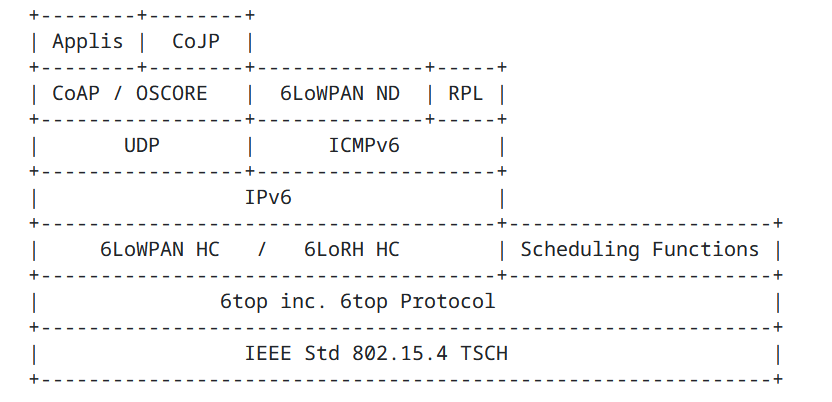
\includegraphics[width=0.7\textwidth]{./images/RFC0768 6TiSCH protocol stack.png}
    \caption{6TiSCH protocol stack defined by RFC9030. \cite{RFC9030}}
    \label{fig:6tisch-protocol-stack}
\end{figure}

The following sections will delve deeper into the most relevant components of the protocol stack defined by \ac{6TiSCH}.



\subsection{\ac{6LoWPAN} Adaptation Layer}
Since IPv6 is built on the assumption that the \ac{MTU} is at least 1280 bytes or above, there is the need to make it compatible with the actual \ac{MTU} of the IEEE 802.15.4 protocol, which is only 127 bytes. In addition the normal IPv6 header size of 40 bytes is too big for such a small data rate, since it alone would already take up around 30\% of the available space.

In order to make IPv6 compatible with IEEE 802.15.4 \ac{6TiSCH} makes use of \acf{6LoWPAN}, which has two main mechanisms for handling the above mentioned problems.
First \ac{6LoWPAN} applies \ac{HC} \cite{RFC6282} to the IPv6 header reducing it from 40 bytes to just a few bytes, by for instance omitting unnecessary or redundant parts of the header. 
Secondly in case a package is bigger than the \ac{MTU} of the link layer \ac{6LoWPAN} handles the fragmentation and reassembly \cite{RFC4944} of data packets. 
By applying these techniques 6LoWPAN makes IPv6, which is primarily designed for comparatively high data rate networks, viable for the IEEE 802.15.4 protocol. 



\subsection{\ac{RPL}}
The \acf{RPL} \cite{RFC6551} is a crucial part of the 6TiSCH stack to ensure reliable and efficient routing in a multi hop and decentralized network. By creating and maintaing a \ac{DODAG} it enables the network to route packets intelligently and efficiently.
The \ac{RPL} root is the central node which coordinates the network and also serves as gateway to external networks. The other nodes in the network communicate upwards to the root via a so called preferred parent, which is determined by listening to \acp{DIO} and according to e.g. link quality pick the preferred parent.
In the joining process of a new node RPL also plays a vital role. One of the first actions the new node does is to listen to \acp{DIO} and then choose it's preferred parent. Having done that the node then is able to send and recieve IPv6 packets.
As can be seen in Figure \ref{fig:rpl-dodag} the nodes are classified into ranks depending on their distance to the sink. Not ony do parent nodes send \acp{DIO} downstream, but \ac{DAO} messages are used by the child nodes to advertivse routes from the leave or intermediate node to the root. These messages inform the root about the structure of the \ac{DODAG} and help to keep it updated.

\begin{figure}[H]
    \centering
    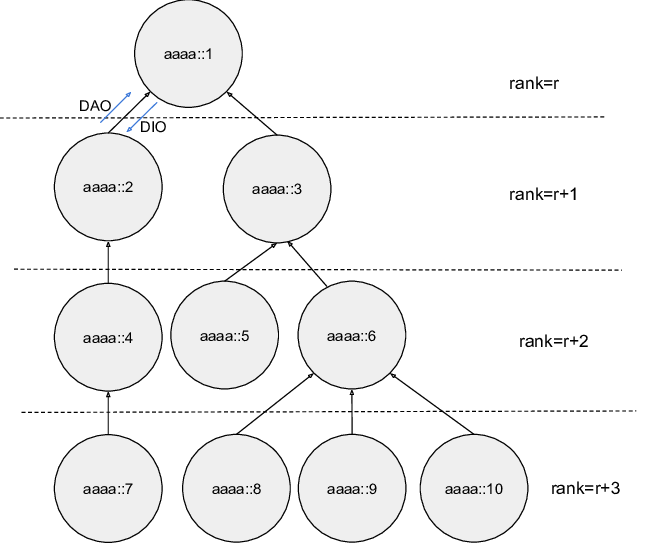
\includegraphics[width=0.7\textwidth]{./images/rpl dodag.png}
    \caption{RPL DODAG showing rang and messages. \cite{rpldodag}}
    \label{fig:rpl-dodag}
\end{figure}



\subsection{\acf{6top} and \acf{6P}}
The so called \ac{6top} \cite{RFC8480} is the connecting layer between the IEEE 802.15.4e MAC protocol and the 6LoWPAN implementation of IPv6. It is the main contribution of the \ac{6TiSCH} protocol and it provides the tools to manage the \ac{TSCH} schedule in a centralized or decentralized manner. It is comprised of two major components firstly the \acf{6P} \cite{RFC8480}, which is a protocol for negotiating cells between nodes and synchronizing the schedules and secondly the \ac{SF} which runs on each node and is responsible for deciding when to add, delete or relocate cells. Cells are categorized into hard and soft cells. Hard cells cannot be changed by \ac{6top} whereas soft cells can be managed by \ac{6top}.

\begin{table}
    \centering
    \caption{6P commands as defined by RFC8480 \cite{RFC8480} taken from \cite{sixpImplementationContiki}}
    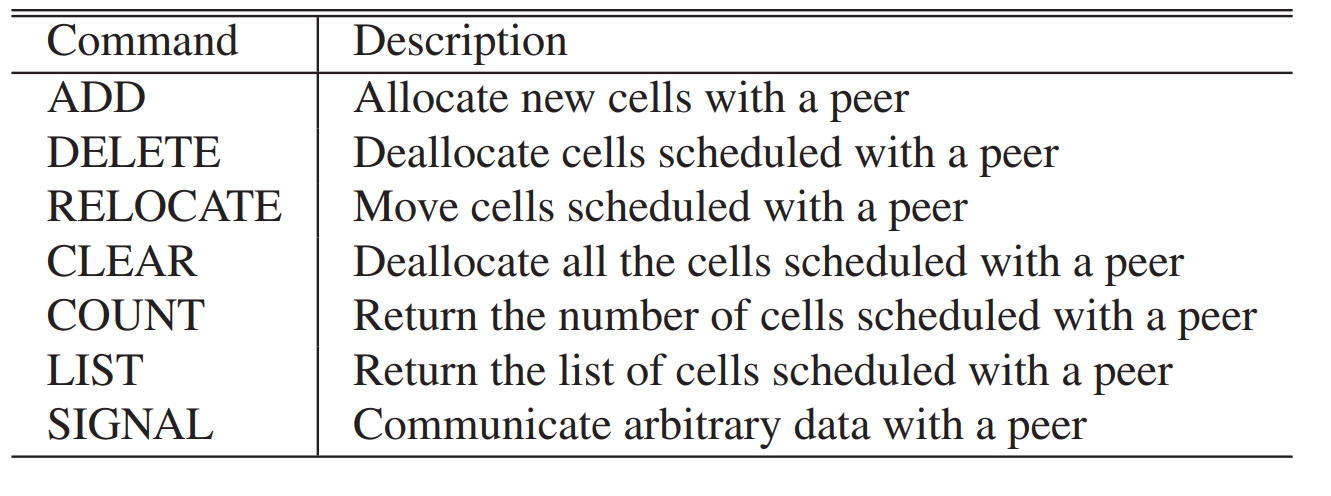
\includegraphics[width=0.7\textwidth]{./images/sixp-commands.png}
    \label{tab:6P-commands}
\end{table}
The \ac{6P} provides several message types for two nodes to negotiate, manage and synchronize their \ac{TSCH} schedule. The available \ac{6P} commands and their functions are listed in Table \ref{tab:6P-commands}. Using \ac{6P} commands the so called \ac{6P} transactions can be made between two nodes for example to add cells to the schedule. \ac{6P} defines two variants of the \ac{6P} add transaction, which are the two way and the three way handshake. For this thesis only the two way handshake will be relevance hence we will only be considering this variant of transaction.
For the \ac{6P} add transaction first an add request is sent by node A containing a list of candidate cells and the amount of cells that the node wants to schedule for communication. Upon recieving the request node B then evaluates which cells are preferred for communication and then sends a response back to node A containing whether the cell allocation has been successful and if yes which cells are allocated.
In case of an error or package loss \ac{6P} also has mechanism in place such as squence numbers and timeouts in order to identfy and deal with errors.

\begin{figure}
    \centering
    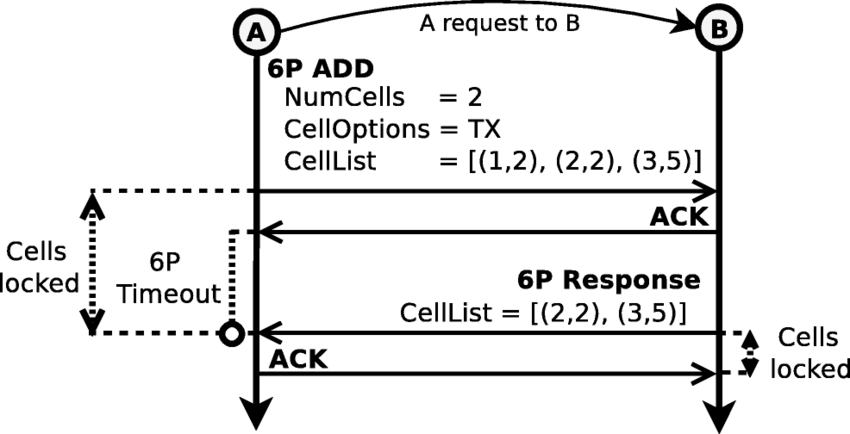
\includegraphics[width=0.7\textwidth]{./images/sixp-add.png}
    \caption{Process of two way 6P ADD transaction. \cite{sixp-add-picture}}
    \label{fig:sixp-add}
\end{figure}


\ac{6top} only defines the mechanism by which the cells are allocated, but it doesn't specify when, how many and which cells are added or deleted for instance. In other words it only provides a framework to manage the schedule, but intentionally leaves the actual implementation of how to manage the schedule undefined. This is due to the different needs of different applications that prioritize different \ac{KPI} and therefore prefer different ways to mangage the schedule. The before mentioned \ac{SF} is the entitiy that takes care of this task and beyond it's tasks is not further defined in the \ac{6TiSCH} specifications.



\subsection{\acf{MSF}}
One such \ac{SF} is the \acf{MSF} \cite{RFC9033ForMSF}, which is a simple and decentralized approach to managing the \ac{TSCH} schedule. It is also the only \ac{SF} to be defined by a RFC making it widely used and researched. 

\ac{MSF} defines three different types of cells for communication.
First it introduces a shared cell typically in the first slot of each slotframe, which is called the minimal cell. This cell is implemented by default and is used for \acp{EB}, \ac{RPL} control messages or join requests from new nodes. 

Second MSF defines autonomous cells, that act as default cells to bootstrap unicast communications. Every node has a permanent Rx autonomous cell whose location in the slotframe is derived from Equation \ref{eq:msf-autonomous-cells-slot} calculating the slotOffset by \ac{SAX} hashing \cite{SAXHashing} the 64-bit \ac{EUI64} of the node and Equation \ref{eq:msf-autonomous-cells-channel} calculating the channelOffset also by hashing the 64-bit \ac{EUI64}. The slotOffset is incremented by one to avoid it interfering with the minimal cell and both hashing computations are limited by the second input given in the hash function, to not exceed the the amount of available timeslots or frequency channels. On this shared cell the children of the node then if needed can schedule Tx cells to the parent and send traffic.

\begin{equation}
    \text{slotOffset}(\text{MAC}) = 1 + \text{hash}(\text{EUI64}, \text{length}(\text{Slotframe\_1}) - 1)
    \label{eq:msf-autonomous-cells-slot}
\end{equation}

\begin{equation}
    \text{channelOffset}(\text{MAC}) = \text{hash}(\text{EUI64}, \text{NUM\_CH\_OFFSET})
    \label{eq:msf-autonomous-cells-channel}
\end{equation}


Third there are negotiated cells which are dedicated unicast cells between two nodes that can be dynamically added or deleted according to the current traffic load.
For the negotiated cells \ac{MSF} has several mechanisms in place to manage the adding, deletion, relocation and synchronization. These mechanisms are governed by several parameters, of which the recommended values are listed in Table \ref{tab:msf-recommended-values}.
\begin{table}
    \centering
    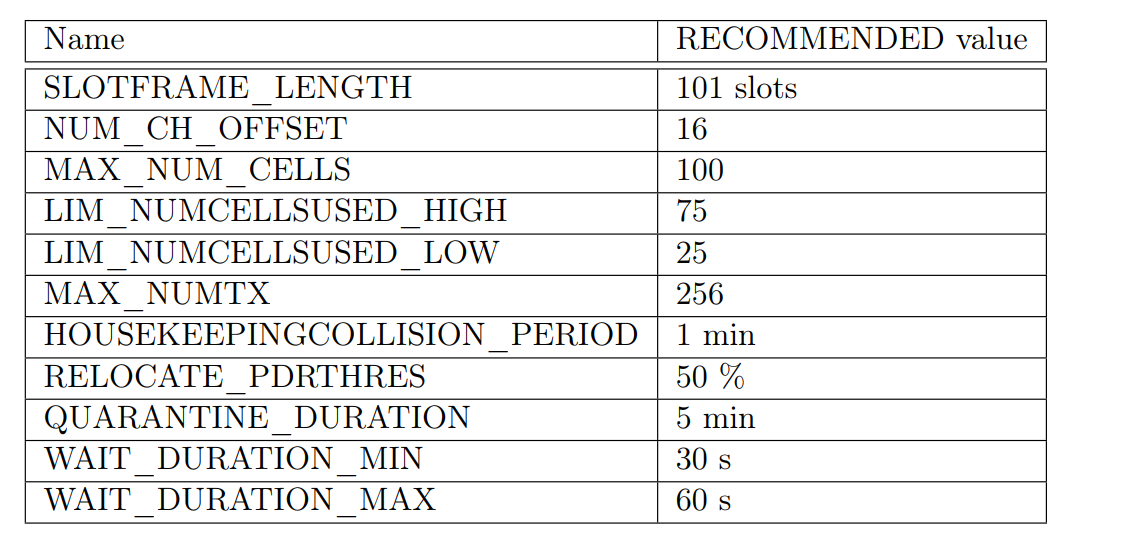
\includegraphics[width=0.7\textwidth]{./images/MSF recommended values .png}
    \caption{MSF recommended parameters RFC9033. \cite{RFC9033ForMSF}}
    \label{tab:msf-recommended-values}
\end{table}

Crucial for the decision making of the \ac{MSF} is MAX\_NUM\_CELLS, which defines the length of the observation window. When NumCellsElapsed, which is the number of negotiated cells that have passed, has reached the value of MAX\_NUM\_CELLS, then the variable NumCellsElapsed is set to zero and the state of the network is evaluated and according to that analysis actions are taken.
In order to decide whether to add or delete cells MSF evaluates the variable NumCellsUsed which keeps track of all the negotiated cells used in the period since the last reset. If NumCellsUsed is above LIM\_NUMCELLSUSED\_HIGH one cell is added. In case it is lower than LIM\_NUMCELLSUSED\_LOW one cell is deleted.

After each HOUSEKEEPINGCOLLISION\_PERIOD \ac{MSF} uses the \ac{PDR} of each negotiated cell to evaluate whether relocation of these cells due to interference or multipath fading is necessary. The necessity of a relocation is assesed by applying the following equation to each cell

\begin{equation}
    PDR_{\max} - PDR_i  > \text{RELOCATE\_PDRTHRES}
	\label{eq:relocation}
\end{equation}

where $PDR_{\max}$ is the PDR of the cell with the highest PDR, $PDR_i$ is the PDR of the cell we are currently evaluating and $RELOCATE\_PDRTHRES$ being the threshold parameter defined in \ac{MSF} which determines when a cell is relocated. If this equation is true then the PDR of the current cell we are evaluating is too low meaning that interference on this cell is likely leading to MSF relocating that cell using a \ac{6P} relocate request.

Using \ac{MSF} as scheduling function the boostrapping phase of the network works as follows. First the manually set \ac{TSCH} coordinator starts up and sends periodic \acp{EB} which contain information about the schloframe length, channel hopping sequence and the \ac{ASN}. Upon receiving a \ac{EB} a node attempting to join synchronizes its clock to the networks schedule, aligning with the \ac{TSCH} timeslot structure. Then initial slots are allocated in the node attempting to join, such as the minimal cell and autonomous cells. Communicating on these cells the node configures its preferred parent via \ac{RPL} with DOI messages. Once the node has joined the \ac{DODAG} it has full connectivity with the network and can now using \ac{MSF} dynamically negotiate cells with its parent.


\subsubsection*{ Cell allocation with sensing }
\label{sec:cell-allo-with-sensing}
In the RFC for \ac{MSF} \cite{RFC9033ForMSF} the sensing cell allocation mechanism is described as an optional extention of the cell allocation mechanism. It suggests a sensing approach to the cell list compilation for the 6P add request where \ac{MSF} creates and maintains a list of candidate cells that are then used as the cell list for cell allocations. On these candidate cells the \ac{MSF} installs Rx cells to monitor for IEEE802.15.4 traffic and if traffic is sensed then the cell is removed from the candidate cell list and a new cell is randomly chosen.





\chapter{Related Work}\label{chp:related}
Concerning the research done in this field concerning \ac{6TiSCH} and \ac{MSF} the overwhelming majority of it is either of analytical or simulation based nature. They evaluate common \acp{KPI} such as end-to-end delay, \ac{PDR} or network adaptation time. Since for meaningful results in experimental validation hardware needs to be configured correctly, enough nodes arranged and many iterations done which is tedious and time consuming many researchers in order to validate their analytical models tend to turn to simulations. Since these can be automated and run in a fraction of the time of experiments they can save a lot of time but still provide support for the mathematical models.


\section{6TiSCH Minimal Scheduling Function: Performance evaluation}
In this paper \cite{MSFPerformanceEvaluation} the authors recommend values for the MSF parameter MAX\_NUM\_CELLS based on simulation results for different network scenarios. The goal is to find suitable values, that increase the adaptability of the network and reduces the 6P control traffic overhead.
In addition, the paper also proposes an improved version of MSF, which is implemented and tested in simulations.

For the simulator they implemented the whole 6TiSCH protocol stack in python and constructed a linear 4 hop topology using 5 motes. For each scenario the simulation was run 1000 times with values for MAX\_NUM\_CELLS= 4,8,16,32. As relevant Key Performance Indicators (KPI) the number of 6P messages sent by each mote and the end-to-end latency of each packet was considered, in order to evaluate which value for MAX\_NUM\_CELLS is the optimal.

For periodic traffic in which each mote generates one packet per slotframe the result was, that the lower MAX\_NUM\_CELLS was chosen, the higher the 6P control traffic overhead was. At the same time the end-to-end delay was little influnced by the change of MAX\_NUM\_CELLS, since MSF already prepares cells in case traffic load increases. As a result of these findings the suggested equation for periodic traffic to calculate the value of MAX\_NUM\_CELLS is:
\begin{equation}
    MAX\_NUM\_CELLS \geq 2  (L  \div 50\%) = 4 L
	\label{eq:max-num-cell-recommended}
\end{equation}
with L being the traffic load of packets per slotframe and 50\% the average cell usage.

For bursty traffic the a similar pattern is observed in which the lower the value for MAX\_NUM\_CELLS the higher the 6P control traffic overhead with small improvements of the end-to-end delay.

Considering the amount of 6P control traffic using MSF, since it can only add or delete one cell at a time the authors suggested an advanced version of the MSF (A-MSF) where the amount of cells to be added or deleted is dynamically calculated. For the amount of cells to add the following equation is suggested:
\begin{equation}
    \text{X} = \text{numTxCellScheduled} (2 \text{cellUsage} - 1)
	\label{eq:improved-msf-add-cells-amount}
\end{equation}
with numTxCellScheduled being the cells scheduled in the last housekeeping period and cellUsage defined as the cells used in that same period.
For the amount of cells to be deleted they suggested this:
\begin{equation}
    \text{X} = \text{numTxCellScheduled} (1 - 2 \text{cellUsage})
	\label{eq:improved-msf-delete-cells-amount}
\end{equation}
With these improvements the authors found that the network improves in 6P control taffic overhead for low MAX\_NUM\_CELLS values while maintaining the end-to-end delay. 


\section{IMSF: Improved Minimal Scheduling Function for Link Scheduling in 6TiSCH Networks}
For this paper \cite{IMSF} the authors suggest an improved MSF where they aim to cut 6P control traffic, packet loss and end to end delay.

The authors identify two major problems of the MSF algorithm which are first, that it only has a reactive mechanism to traffic change. Meaning that the system always lags behind the actual number of cells needed for the network to be most efficient. Second the MSF is not flexible in the number of cells it adds/delets, when it senses a change of traffic. This is especially inefficient when there is a sudden spike in traffic, which would require the network to provide high amounts of cells to be added quickly.

With this in mind they suggest an improved minimal scheduling function (IMSF), which estimates the expected NumCellUsed i.e. the future traffic demand, calculates the cells needed to be added/deleted and then sends a single 6P add/remove request based on the results of the calculation. 

To calculate the estimated amount of cells to add they suggest this equation:
\begin{equation}
    0.25 < \frac{T(i,A) ETX}{16(len(Tx_CE LLS)+x)} \le 0.75
	\label{eq:imsf-estimated-cells-add}
\end{equation}
with Expected Transmission Count (ETX) and .... as the queued packets already existing in that node.

In order to calculate the estimated amount of cells to delete they use this equation:
\begin{equation}
    y=\lfloor len(Tx_CE LLS)(\frac{ 0.75 - Cell _utilization}{0.75}) \rfloor
	\label{eq:imsf-estimated-cells-delete}
\end{equation}

To test the IMSF a python based open-source simulator for 6TiSCh networks was used to simulate three different network topologies, varying amounts of nodes and with bursty and periodic traffic. The results are, that the IMSF consistently outperforms the default MSF and A-MSF, which has been suggested in the paper \cite{MSFPerformanceEvaluation} detailed above. Under different network conditions it can be observed, that 6P control traffic overhead and also end-to-end delay have been significantly decreased.


\section{Pushing 6TiSCH Minimal Scheduling Function (MSF) to the Limits}
In order to gain a deeper understanding on 6TiSCH MSF on a fundamental level the authors of this paper \cite{PushingMSFToTheLimits} have simulated a network with constant and varying traffic to figure out how effective MSF's adaptation mechanisms are. For their python based simulation \cite{Simulating6TiSCHNetworks} they implemented a 5 node linear topology with the standard recommended values for MSF. For the data collection node 2 was chosen due to the fact, that all the traffic from the nodes before pass through this node.

Firstly they examined the behaviour of the network under constant traffic and how it adapts to the initial change and then stabilizes. One of the main findings w as, that the lenght of the cell allocation period has a major affect on the PDR of the network as can be seen in figure \ref{fig:6p-add-time-length-relation-pdr}. That is because in that period the packet queue of a node fills up, since there is not enough cells per slotframe to handle the increased traffic, and at a certain point when the queue is full packets then are dropped. Another pattern that was observed was, that with higher traffic rates the PDR increased while the latency decreased. This counter-intuitive result comes from the fact, that with more traffic also more cells are allocated making it more likely for a packet to have a close cell cell scheduled in which it can be sent immediately after arriving at a node. 
\begin{figure}
    \centering
    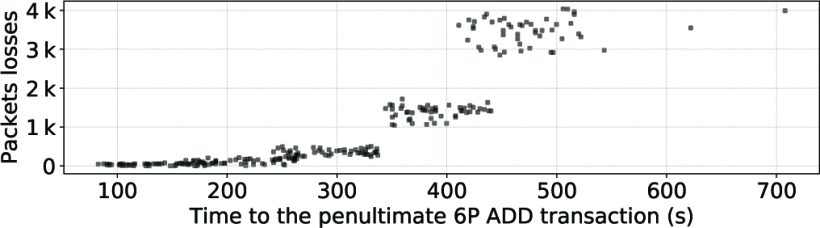
\includegraphics[width=0.7\textwidth]{./images/pushing 6tisch msf to the limits - 6p add length time graph.png}
    \caption{Packet loss in relation to time it takes for the constant traffic network to stabilize.}
    \label{fig:6p-add-time-length-relation-pdr}
\end{figure}

Secondly a network with periodic change in traffic was simulated and observed. The main objective was to easure the time period from when the packet rate change to when the schedule reached a stable state. It took the longest in the beginning of the network, since there were little cells to send communication traffic on resulting in the allocation process to take very long. But with increased traffic the time to allocated then stayed roughly the same as can be observed in figure \ref{fig:6p-add-time-length-relation-pdr-dynamic}.
\begin{figure}
    \centering
    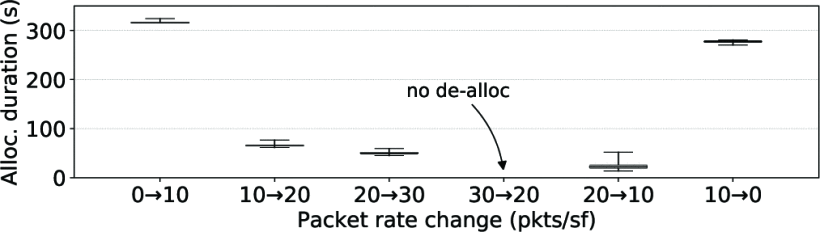
\includegraphics[width=0.7\textwidth]{./images/pushing 6tisch msf to the limits - 6p add length time graph (dynamic traffic).png}
    \caption{Time of adaptation for each traffic change.}
    \label{fig:6p-add-time-length-relation-pdr-dynamic}
\end{figure}

This paper gives a good first impression on the effectiveness of the adaptation mechanisms of 6TiSCH MSF and shows the importance of the cell allocation time as a key performace indicator (KPI), directly affecting the PDR.


\section{Thorough Performance Evaluation \& Analysis of the 6TiSCH Minimal Scheduling Function (MSF)}
In this paper \cite{sixp-add-picture} David Hauweele et al. the authors of \cite{PushingMSFToTheLimits} mentioned in the previous section expanded their work on \ac{6TiSCH} \ac{MSF} evaluation by studying the behaviour and reactivity of the network under varying traffic loads and proposing a mathematical model in oder to predict the convergence pattern of \ac{MSF}.
The evaluations made in the same python based simulator were conducted on a linear topology with constant and varying traffic loads. Results show that the more cells are allocated the faster \ac{MSF} adapts to changing traffic. It was observed that at higher traffic loads \ac{MSF} tends to overprovision while improving latency, since using the recommended values it allocates cells at a 75\% cell utilization but only deallocates cells once cell utilization is below 25\%.
The paper propses following equation
\begin{equation}
    T_{msf}(a, b) = T_{sf} \times \sum_{k=a}^{b-1} \left( \frac{1}{2} + \frac{1}{2k} + \frac{\text{MAX NUMCELLS}}{k} \right)
    \label{eq:t_msf}
\end{equation}

to calculate the time required by \ac{MSF} in order to go from a to b allocated cells. The model multiplies $T_{sf}$ which is the time for a slotframe by the necessary slotframes to allocate all cells. The latter is computed by taking the sum of all slotframes needed for each allocation.

At last the paper investigates the impact of different \ac{MSF} parameters on packet losses and resource utilization. Findings include that by reducing MAX\_NUM\_CELLS faster traffic adaptation by quicker cell allocation can be achieved, due to the shortened period in which traffic load is evaluated. This however also makes the evaluation less precise since the amount of gathered data is less potentially leading to inefficient allocation patterns.
To limit overprovisioning adjusting the thresholds for cell allocation and deallocation was found to be effective, where a smaller gap between the lower and upper bound reduced overprovisioning while increasing allocations and deallocations. This shows the tradeoff that is to be made between precision in estimating the traffic load and stability, since with the former small changes already trigger allocations or deallocations and with the latter overprovisioning is high.
The paper concludes that improving \ac{MSF} requires modifying the \ac{SF} itself, which for example the A-MSF approach suggests, because attempts to reduce convergence time and limit overprovisioning caused instability in the network.


\section{An Experimental Evaluation of the 6top Protocol for Industrial IoT Applications}
For evaluating 6top and it's performance in a real environment \cite{ExperimentalEvaluationOf6topForIoT} Francesca Righetti et al. set up a experimental testbed of nodes. They had a network of 23 nodes with each being a Zolertia RE-Mote sensor node running on Contiki OS which is a operating system for sensor nodes with built in 6TiSCH implementation. As SF they used On-the-Fly (OTF) \cite{OTFFor6TiSCH}, which allocates cells according to the data traffic demand and Proportional, Integral, Derivative (PID) \cite{PIDBasedScheduling}, which allocates cells according to the queue occupancy.

For the experiments the authors have three metrics to evaluate the performance, which are the success rate, transaction delay and the failure rate. Applying these KPIs the team found that the SF has a big influence on how efficient the 6top layer works. For instance for the success rate of the 6P transactions the failure rate for each tested traffic rate was below 70\% for PID. In contrast to that with the same traffic rates OTF manages to maintain 6P transaction failure rates above 80\%. This is due to the fact that for PID a lot of allocations and deallocations are made, which increase the number of 6P transactions and therefore leading to a high failure rate.
Another finding that is presented is the actual transaction delay that is defined as the time from when the 6P request is send to the time when a response is recieved. In previous papers this time has been assumed as negligible \cite{DecentralizedBroadcastBasedScheduling}, but after real world testing the authors found, that depending on the traffic rate and SF average transaction delays from up to 0.5 seconds to 2.2 seconds can occour.
As main contributing factors to these failures the authors list insufficient resources, 6top timeout expiration, schedule mismatch and buffer overflow.


\section{Decentralized Traffic Aware Scheduling in 6TiSCH Networks: Design and Experimental Evaluation}
In \cite{7254107} Accettura et al. propose the decentralized traffic-aware scheduling (DeTAS) approach, which is the decentralized extention of the traffic-aware scheduling approach (TASA) proposed first by \cite{Palattella2012}. It aims to achieve collision-free schedules in a multihop \ac{TSCH} network by using a small amount of information that is locally communicated between the nodes in order to configure the schedule. DeTAS takes into account the queue levels thereby avoiding traffic congestion and reducing the possiblity of packet drops due to the queue being full. This traffic information of a node is received from the children and the node itself also passes it's traffic amount up to the parent. From this information the network then can decentrally build up a collision free schedule by allocating transmission and reception cells in a way that ensures nodes with a shared communication space do not transmit at the same time therefor minimizing collisions.

To facilitat the exchange of traffic information among nodes the paper also introduces DeTAS \ac{MAC} command frames. It firstly defines the REQ command, which is sent by a node to its parent with information about it's traffic requesting scheduling information from the parent. Secondly the RES command is sent as a response by the parent in order to provide the requested scheduling parameters to the child node.

With DeTAS implemented in the OpenWSN \cite{Watteyne2012} project a open source implementation of standard communication protocols such as \ac{TSCH} and \ac{RPL} the authors used TelosB motes to experimentally validate it's performance. Two different network topologies were implemented namely a double chain topology evaluating network depth and a binary tree topology assessing performance in dense networks. As \ac{KPI} end-to-end delay, link packet loss ratio (PLR) and node duty cycle were considered.

In the experiments on the double chain topology it was found that with increased distance to the root node the duty cycle decreased, since the nodes closer to the root thus acting as traffic bottlenecks while end-to-end delay increases. With a increased number of channel offsets the duty cycle, interference and end-to-end delay were able to be reduced.
For the experiments on the binary tree topology similar results were observed confirming, that DeTAS performs consistently across various topologies.

The paper provides a decentralized approach to scheduling in \ac{6TiSCH} and validates it's proposal with experimental tests showing the value of an experimental approach to validating performance of scheduling approaches.

\section{Novelty}
The research into \ac{MSF} has been quite deep from a theoretical point of view and many aspects such as the ideal amount of cells to add, best \ac{MSF} parameters to choose for a desired behaviour and overprovisioning have been studied in depth. Using models and validating them with simulations a good understanding of \ac{MSF} has been gained also leading to suggestions of improvement such as with the A-MSF  \cite{MSFPerformanceEvaluation} or IMSF \cite{IMSF}.
Although the cell allocation process has been part of some of the above mentioned works the mechanism for which cells to include into the cell list of a \ac{6P} add request has not been evaluated at all. In addition to that none of the \ac{MSF} focused works have used experimental methods to validate their findings showing that there is a lack of experimental approaches when it comes to studying \ac{MSF}.
Taking that into account the following sections attempt to present a analytical model for the cell allocation time taking into account the cell list selection mechanism and integrating the sensing improvement which was suggested in the RFC. The provides a deeper understanding of the cell allocation mechanism and seeks to offer insight into what could be more effective ways of compiling a \ac{6P} add cell list.
Furthermore the results are validated by conducting experiments and discussing them alongside the analytical results.


\chapter{Analytical Model}\label{chp:model}
The analytical model developed and outlined in this work assumes a two node network consisting of parent and child and additional an network with constant traffic rate. The scope of the analysis focuses on the cell allocation period and does not include the bootstrapping phase of the network.
As \ac{KPI} we consider the time it takes for the schedule to reach a stable state and the probability of cell overlap, since they best capture a holistic performance of the scheduling function and it's subsequent cell allocation mechanism.

\begin{figure}[H]
    \centering
    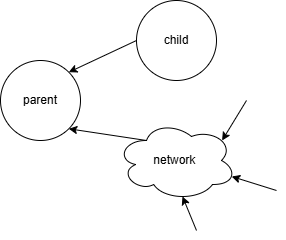
\includegraphics[scale=0.7]{./images/network_outline.png}
    \caption{Network topology assumed by the model}
    \label{fig:analytical-network-model}
\end{figure}


\section{ Default Cell Allocation Mechanism }
In order to determine how effective a certain cell allocation mechanism is we consider the time it takes for a network to reach a stable state after adapting to a constant traffic rate of $\lambda$ which is being served by allocating $\mu_{\max}$ amount of cells. The network is considered stable if all cells have been evaluated in terms of \ac{PDR} and none have been determined to be in need of further relocation. 
The cell allocation mechanism mostly affects the time it takes to allocate a certain amount of cells and the quality of the cells, meaning how much interference there is on them. For this reason using scheduling time as \ac{KPI} is an effective way to measure the performance of the cell allocation mechanism, because more low quality cells also means more relocations needed, resulting in an overall longer time until the network is stable. 

The time $T_s$ it takes for a network to reach a stable state is calculated by:

\begin{equation}
    T_s = T_a + T_r
    \label{eq:t_s}
\end{equation}

where $T_a$ is the time it takes to allocated all $\mu_{\max}$ cells and $T_r$ is the time it takes for all of the cells to be relocated until there is no relocation necessary.


\subsection{ Cell Allocation Time }
The time to allocate $\mu_{\max}$ cells is calculated as follows:
\begin{equation}
    T_a = \sum_{i=2}^{\mu_{\max}} \left( \frac{M}{i - 1} + \frac{1}{i} + 0.5 \right)
    \label{eq:t_a-allocation-time}
\end{equation}

where we take the sum of the time it takes to allocate each cell until we reach $\mu_{\max}$ cells, which is derived from the target traffic rate $\lambda$ (packets per \ac{SF}) defined by the application and is calculated as:

$$\mu_{\max} = \left\lceil \frac{\lambda}{u_{high}} \right\rceil$$ 

with $u_{high}$ being the upper cell utilization threshold in \ac{MSF} which determines at what cell utilization threshold another cell is added.
For this model we start at the second cell since the mechanism for the allocation of the first cell in \ac{MSF} is a special case that counts autonomous cells into the NumCellsElapsed which normally only keeps track of negotiated cells and not autonomous cells. So for the sake of simplicity and generality we leave out the allocation of the first cell and consider it from there onwards.

For each cell allocation we first need to wait for \ac{MSF} to recognize that a cell allocation is necessary. This happens every time the number of elapsed cells reaches MAX\_NUM\_CELLS. By dividing MAX\_NUM\_CELLS by the amount of cells already scheduled we can get the time it takes for \ac{MSF} to initiate another cell allocation.

Secondly we need to factor in the time it takes for the 6P ADD request to be sent and for the response to be received. Considering \cite{Tasixptransactiontime} and adapting the models to our case the second addend models the mean waiting time to the next scheduled cell with $\mu_i - 1$ cells, since $\mu_i$ is the cell which we are trying to allocate but hasn't been allocated yet. 
At last the third addend in this sum accounts for the waiting time of the 6P RESPONSE to the next scheduled cell in the parent node. This stays constant, since we assume that the parent node only communicates via the autonomous cell to the child node.


\subsection{ Cell relocation time }
Assuming recommended values for the \ac{MSF} \ac{SF} presented in Table \ref{tab:msf-recommended-values} the cell relocation time is calculated as


\begin{equation}
    T_r = t_h \min(\lfloor E_\Sigma[O] \rfloor, 1) + \left(\frac{1}{\mu_i} + 0.5\right) \left\lceil \frac{\lfloor E_\Sigma[O] \rfloor}{r_l} \right\rceil
    \label{eq:analytical-T_r}
\end{equation}

where the first addend models the time it takes for \ac{MSF} to evaluate the cell performance and, if needed, initiate a cell relocation. The second addend models the time it takes for the \ac{6P} RELOCATE requests and responses to be exchanged.

In order to calculate $t_h$, which is the time it takes for \ac{MSF} to evaluate all cells we can use the following equation:

\begin{equation}
    t_h = \left\lceil\frac{MAX\_NUMTX t_{slotframe}}{t_{housekeeping}}\right\rceil t_{housekeeping}
    \label{eq:analytical-t_h}
\end{equation}

Since only after a cell has been used for MAX\_NUMTX times and the value has been halved it will be evaluated for relocation we multiply the amount of times the cell needs to be used by the time it takes for a slotframe to pass $t_{slotframe}$. Then we take the rounded up value of that product  and divide it by $t_{housekeeping}$ which is the HOUSEKEEPINGCOLLISION\_PERIOD. This yields the number of HOUSEKEEPINGCOLLISION\_PERIODs we need to wait for the cells \ac{PDR} to be evaluated for relocation. To obtain the actual time we then at last multiply it by $t_{housekeeping}$.

To model the likelihood of a relocation to occur we first consider the probability from a node's perspective for a cell that it is about to allocate to overlap with the cells that already are occupied by neighbors in its communication range. For a network with constant traffic of N cells per slotframe and X being the total amount of cells available in the network the probability of a cell overlap of the i-th cell allocated is calculated by:

\begin{equation}
    p_{ov} (\mu_i) = \frac{N}{X-\mu_{i-1}}, \quad X=n_{ch} n_{sf} ,
    \label{eq:analytical-p_ov}
\end{equation}

where X is computed by the product of available channels and timeslots in a slotframe.

In order to quantify from this how many relocations on average are needed we can calculate the sum of expected cell overlaps like in Equation \ref{eq:t_a-allocation-time} from the second allocated cell to $\mu_{\max}$ by

\begin{equation}
    E_\Sigma[O] = \sum_{i=1}^{\mu_{\max}} \frac{p_{ov}(\mu_i)}{1 - p_{ov}}
    \label{eq:analytical-E_sigma(O)}
\end{equation}

Assuming that if multiple relocations are necessary they are all done in the same HOUSEKEEPINGCOLLISION\_PERIOD we only need to consider this value until it is >= 1, which is also the reason why for Equation \ref{eq:analytical-T_r} we take the minimum of $E_\Sigma[O]$ and 1.


The second addend in Equation \ref{eq:analytical-T_r} calculates the time it takes for the individual requests to be sent and the respective response to be received. Similarly to calculating the cell allocation time we can rely on the work done in \cite{Tasixptransactiontime} to estimate the time for these messages to be sent. In order to account for multiple \ac{6P} RELOCATE requsts we multiply the time it takes for the messages to be sent by the rounded up value of $E_\Sigma[O]$ the expected amount of relocations divided by $r_l$ - the limit of relocations per message. To calculate $r_l$ we consider the MTU of IEEE 802.15.4 and the standards defined by \cite{RFC8480} regarding the \ac{6P} RELOCATE request:

\begin{equation}
    r_l=  \left\lfloor \frac{P_{\max}}{(\eta + 1)c} \right\rfloor, \quad \eta \geq 1 
    \label{eq:analytical-relocation-maximum}
\end{equation}

With $P_{\max}$ being the the available payload size without header in bytes, $c$ the size of a cell in bytes and $\eta$ the redundancy constant which ensures that for each cell relocated at least two candidate cells are included.
Plugging in the standard values for a \ac{6TiSCH} network and with a minimum $\eta$ of 1 we get a maximum of 12 cells per relocation request.


\section{Cell Allocation Mechanism with Sensing}
\label{sec:cell-alloc-mech-sens}
The sensing approach studied here is based off the suggestion from \cite{RFC9033ForMSF} described in Section \ref{sec:cell-allo-with-sensing}, but with some adjustments.
The cells in which traffic is sensed and that are being removed from the candidate cell list will be put on a blacklist to prevent them from being chosen again. In this manner we have a list of cells which we are confident in having next to no interference and a list of cells where we know that there is interference.

With this sensing approach we now only consider the probability of overlap for the cells in the candidate list, since they are the only ones used to compile the cell list of the \ac{6P} add request. This set of candidate cells C is chosen from among the pool of all available cells $X'$. Considering this we can calculate the probability of choosing cells in a way that at least one cell is overlapped with following equation:

\begin{equation}
    p_{ov}^{(C)} = 1 - (1 - \frac{N}{X'})^C , \quad X'=X-n_{min}-\mu_i-n_{auto}
\end{equation}

where C is the amount of cells in the candidate cell list and $X'$ being calculated by the total amount of cells available minus the amount of scheduled minimal cells $n_{min}$ the amount of already negotiated cells $\mu_i$ and the amount of scheduled autonomous cells $n_{auto}$. The probability of at least one cell in the C candidate cells being overlapped $p_{ov}^{(C)}$ is computed by one minus the probability of all cells chosen not being overlapped.

Over time with sensing the cells and replacing the ones with sensed overlap the list of candidate cells will be overlap free. The time it takes to sense all the cells in the candidate list $t_s$ is determined by the amount of sensing operations done and the amount of sensing operations needed to sense all the overlapped cells. The minimum amount of sensing operations needed to ensure no overlap is computed by

\begin{equation}
    n_{s\_min} = \lceil Cp_{ov}^{(C)} \rceil \zeta \quad ,
\end{equation}

where $\zeta$ is the redundancy factor describing how many times a cell must be sensed with no traffic detected in order to have the confidence that it is not overlapped.
Similarly we can also compute the maximum and the average amount of sensing operations needed in order to have confidence in all C candidate cells.

\begin{equation}
    n_{s\_max} = C \zeta
\end{equation}

\begin{equation}
   \bar{n_s} = C(1-\frac{1}{1+\lceil Cp_{ov}^{(C)} \rceil}) \zeta
\end{equation}

Using this we then can calculate the time it takes on average for the candidate cell list to be considered overlap free by

\begin{equation}
    \bar{t_s} = \frac{\bar{n_s}}{X_s} \quad ,
 \end{equation}

where $X_s$ is the amount of cells sensed per slotframe.
Considering that using recommended \ac{MSF} values the time it takes to allocate a cell is in the order of tens to hundreds of seconds with reasonable $X_s$ the time $\bar{t_s}$ becomes negelectable. This means that to integrate the sensing mechanism into the model previously introduced in Equation \ref{eq:t_s} we simply assume $p_{ov}$ used in Equation \ref{eq:analytical-E_sigma(O)} to be zero at the time of cell allocation.

The fact that cells allocated with the sensing mechanism have a higher \ac{PDR} leading to less \ac{6P} messages being lost and therefor decreasing the time wasted on waiting for \ac{6P} timeouts and retries was considered. But due to time constraints and the limited scope of this work its effect on $T_s$ was not included in the mathematical model.



\chapter{Experimental validation}\label{chp:implementation}
This chapter goes into detail about the experimental setup, execution of the experiments and a discussion of the results obtained in the experiments compared to the calculations of the analytical model.

\section{Methodology}
In order to experimentally validate the performance of cell allocation mechanisms a setup has been implemented, which models the network topology shown in Figure \ref{fig:analytical-network-model} in which there are two nodes and a neighboring network with constant traffic rate. This network with constant traffic rate is necessary in order to cause cell overlaps resulting in relocations. The coming sections will outline the technologies used to emulate this setup and the methods used for collecting and processing the data.


\subsection{ Openmote-B and Contiki-NG}
As hardware platforms for the experiments we chose the Ultra Low-power Openmote-B board, which has been designed specifically for developing and researching low power wireless networks in the domain of Industrial Internet of Things (IIoT).
The board is based on the Texas Instruments CC2538 \ac{SoC} with integrated 32-bit ARM Cortex-M3 microcontroller. It allows for wireless communication on 2.4GHz and Sub-GHz frequencies via external antennas fully supporting the latest IEEE 802.15.4 standard and features a serial USB-Port connection for flashing and logging.

As operating system for the Openmote-B boards we used the Contiki-NG (Next-Generation) real-time operating system (RTOS). It is a continuation of the popular Contiki-OS improving it in performance, and usability while staying lightweight.
As a open-source operating system it is primarily designed for resource-constrained devices most commonly found in \ac{IoT} with limited memory, processing power and battery life.
The default version of Contiki-NG comes with widespread \ac{IoT} protocols implemented such as \ac{RPL}, IPv6/\ac{6LoWPAN} and  \ac{6TiSCH}. It's compatibility with a wide array of platforms such as the Openmote or the Zolertia Zoul makes it a popular choice for developing low-power wireless applications. 
One of the most unique features of Contiki-NG is the Cooja network simulator that allows for simulation of networks using the above mentioned supported platforms running the Contiki-NG operating system without having the actual hardware. It allows researchers and developers to monitor communication, logs and energy consumption without having to deploy an actual physical setup of the network.

At the core of Contiki-NG lies a event driven system enabled by a event loop that constantly checks for events and then yields control to the process associated with that event. This approach using so called Protoheads as lightweight and stackless threads implements cooperative multitasking. It means that each process voluntarily yields back control to the scheduler. This allows for efficient and low power multitasking without the overhead of context-switching operations usually deployed by preemptive systems.
Applications are implemented in such processes, which become active if the respective event is triggered and then perform the tasks necessary before handing back control.
In Contiki-NG different types of timers provide precise tools for time sensitive applications. Whether the event timer for periodic tasks or the real time timer for high precision timing Contiki-NG provides a simple timer API to initialize, start, stop, reset and read timers. When getting the current system time it returns ticks, which are the CPU clock cycles since the start of the system. In order to obtain the real world time the platform specific CLOCKSECONDS variable can be used which is the ticks per seconds for each platform.

Natively Contiki-NG supports IEEE 802.15.4 and already provides an implementation of the \ac{TSCH} schedule and \ac{6top}-sublayer. In order to implement the modifications necessary for conducting the experiments we need to first have a rough understanding of the inner workings of the \ac{6top} implementation in Contiki-NG. 

\begin{figure}[H]
    \centering
    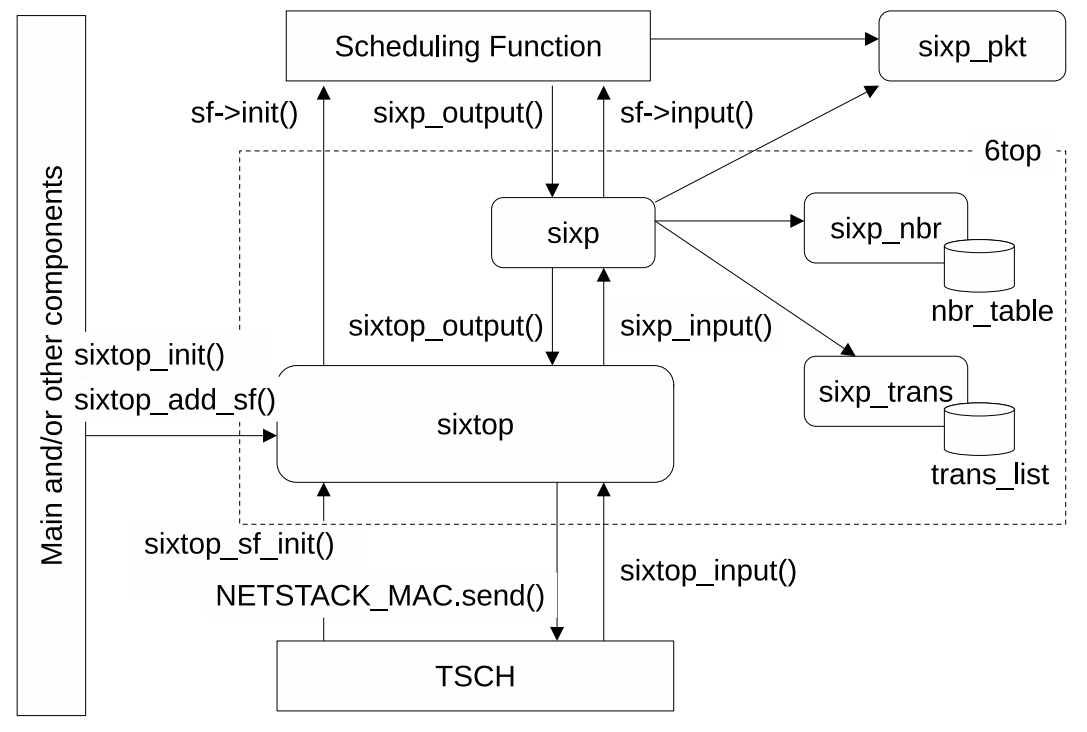
\includegraphics[width=0.7\textwidth]{./images/sixp in contiki.png}
    \caption{\ac{6P} implementation in Contiki-NG. \cite{sixpImplementationContiki}}
    \label{fig:sixp-implementation}
\end{figure}

From this graph it can be seen, that \ac{6top} and it's subsequent sixp module mainly provide \ac{SF} with an interface for outputting \ac{6P} messages via the sixp\_output() function. It keeps track of the neighbors and manages the status of the \ac{6P} transaction ensuring, that only one is currently active.
Additionally when a input is passed down from the \ac{MAC} layer it calls the input function defined by the \ac{SF}.


\subsection{ Data collection }
The data collected for the evaluation was mainly the timing of each cell allocation, cell relocation and information about which cell was relocated. To obtain this data the serial logging function of the Openmote-B boards was used to log the outputs of the cell allocating node. The relevant data was first extracted by a python script and written into a csv format and then further processed and visualized into graphs using a second python script.


\section{Experimental Setup and Application Design}
In order to experimentally validate the analytical model we matched the topology presented in Figure \ref{fig:analytical-network-model} by setting up three Openmote-B nodes that each fulfill one of the distinct roles of that network. In this section the setup will be introduced and the technical details roughly explained. An exemplary view of the experimental setup can be seen in the Figure \ref{fig:experimental setup}. Each experiment was conducted 10 times manually resetting the boards for a new iteration.

\begin{figure}[H]
    \centering
    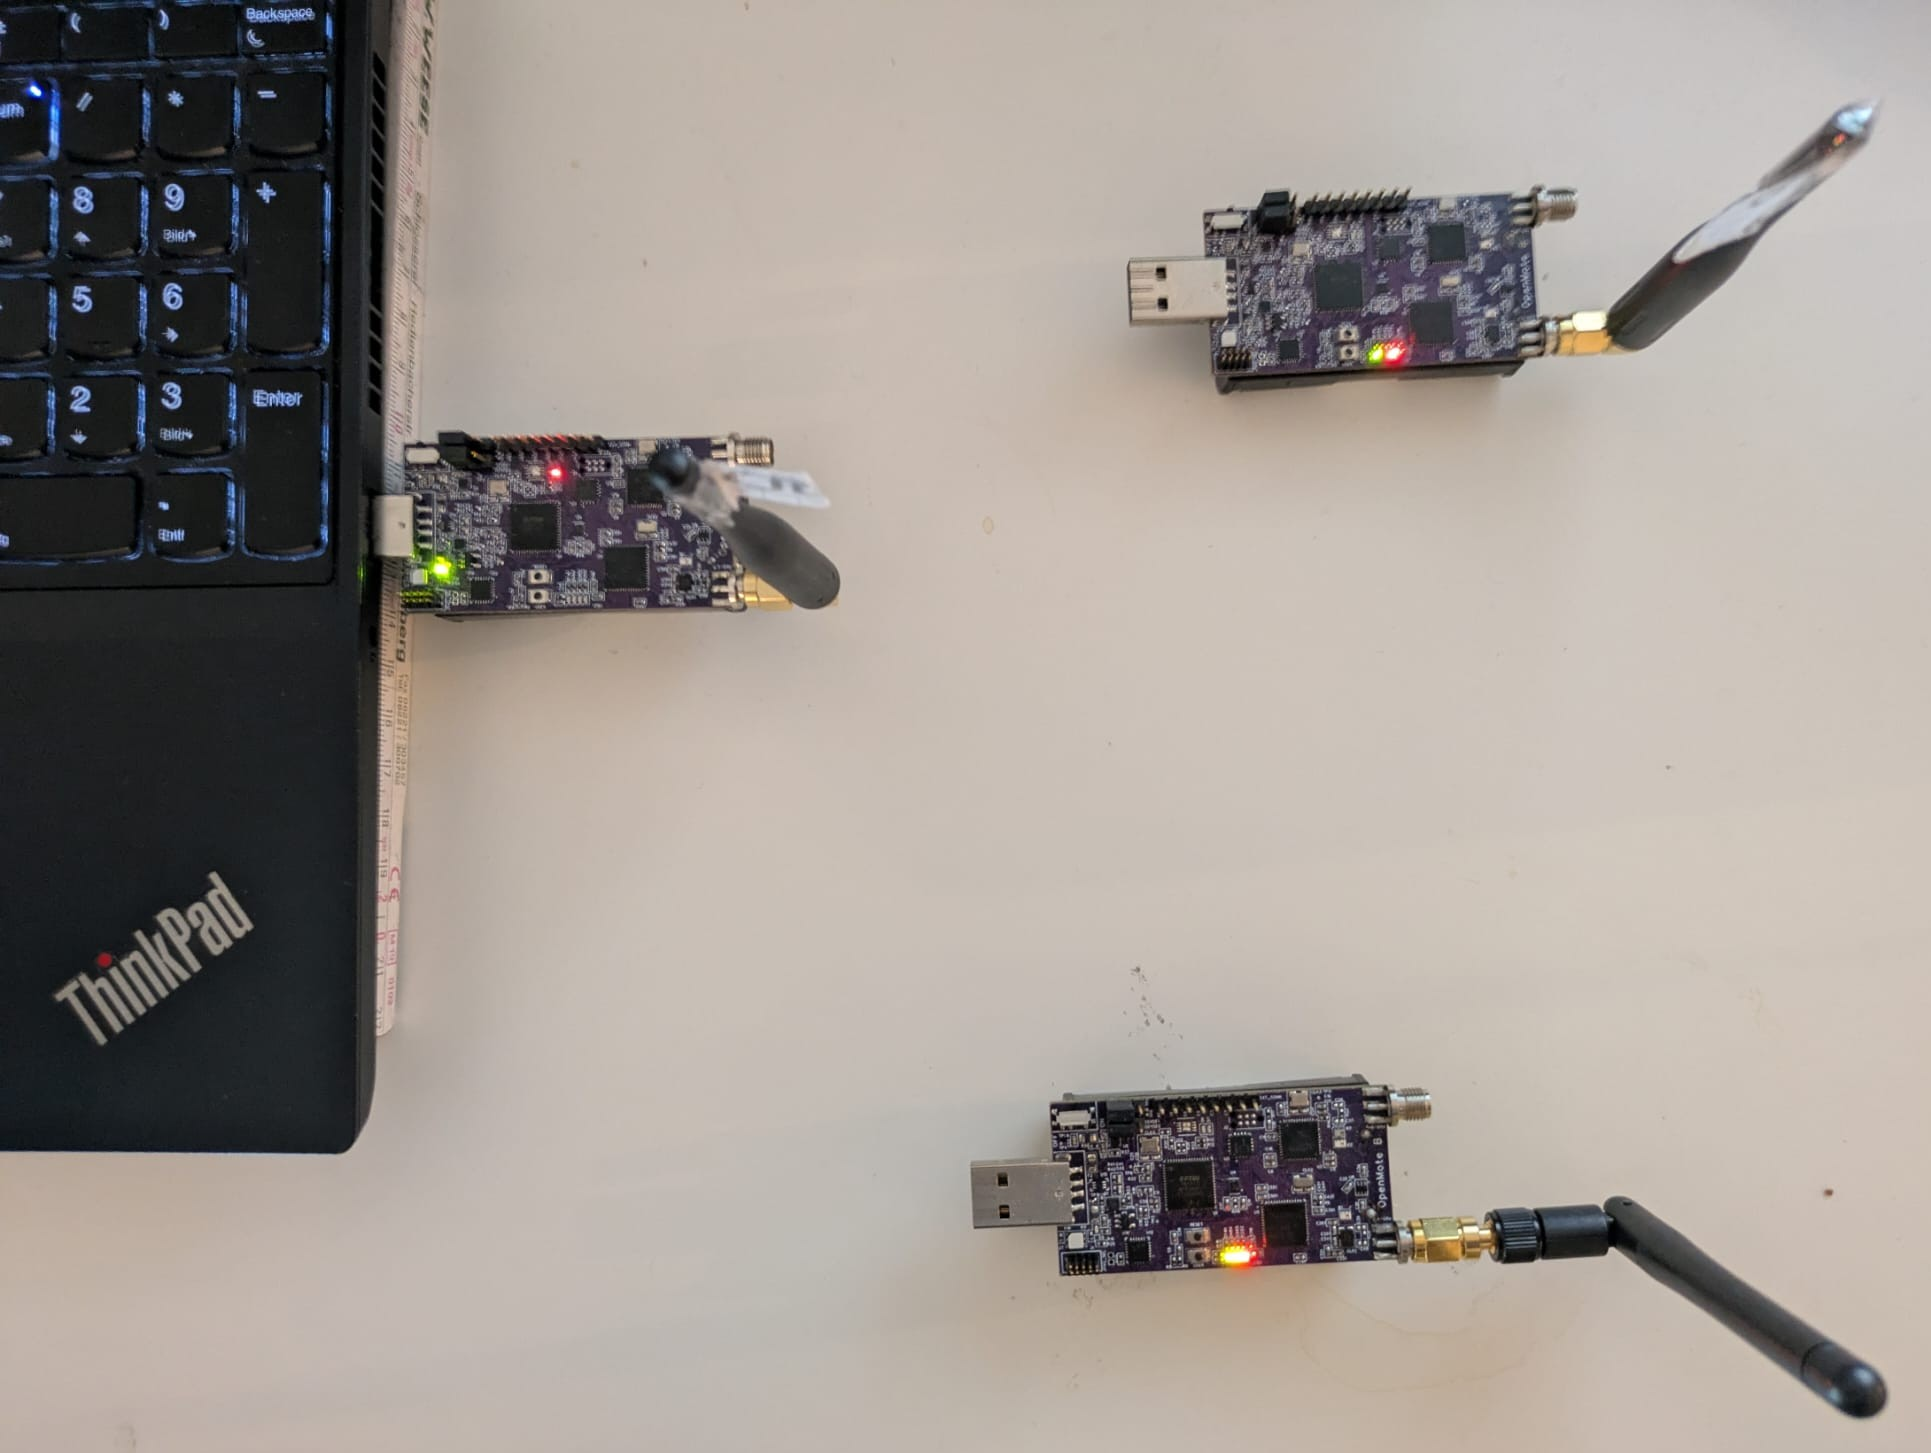
\includegraphics[width=0.7\textwidth]{./images/Setup photo.jpg}
    \caption{Experimental setup.}
    \label{fig:experimental setup}
\end{figure}

The processes on each node are based on a combination of two preinstalled examples of Contiki-NG. The first is the rpl-udp example containing the implementation of a udp client node and a udp server node able to communicate with each other via UDP messages using RPL routing. The second is the sixtop example, which comes with a rudimentary scheduling function handling the addition and deletion of cells. This includes generating and populating requests and responses but also processing incoming ones and taking appropriate action by scheduling or deleting cells in the schedule. For these tasks the \ac{TSCH} API and the \ac{6P} API were used.

\subsection*{Parent Node}
The parent node acting as the \ac{TSCH} coordinator and \ac{RPL} root node is running two processes. The first them sets up the tsch network and responds to any incoming \ac{6top} traffic. The second process initializes a  \ac{UDP} server to process any incoming \ac{UDP} packets. If a message is received the parent node checks whether it is from the network emulator or the child and then if no autonomous cells have been added to that node it will add them. These autonomous cells are set up in order to emulate the autonomous cells in \ac{MSF} with the difference that the timeslot and channeloffset of these cells are hard coded and not calculated using the standard defined in Equation \ref{eq:msf-autonomous-cells-slot} and \ref{eq:msf-autonomous-cells-channel}.

\begin{figure}[H]
    \centering
    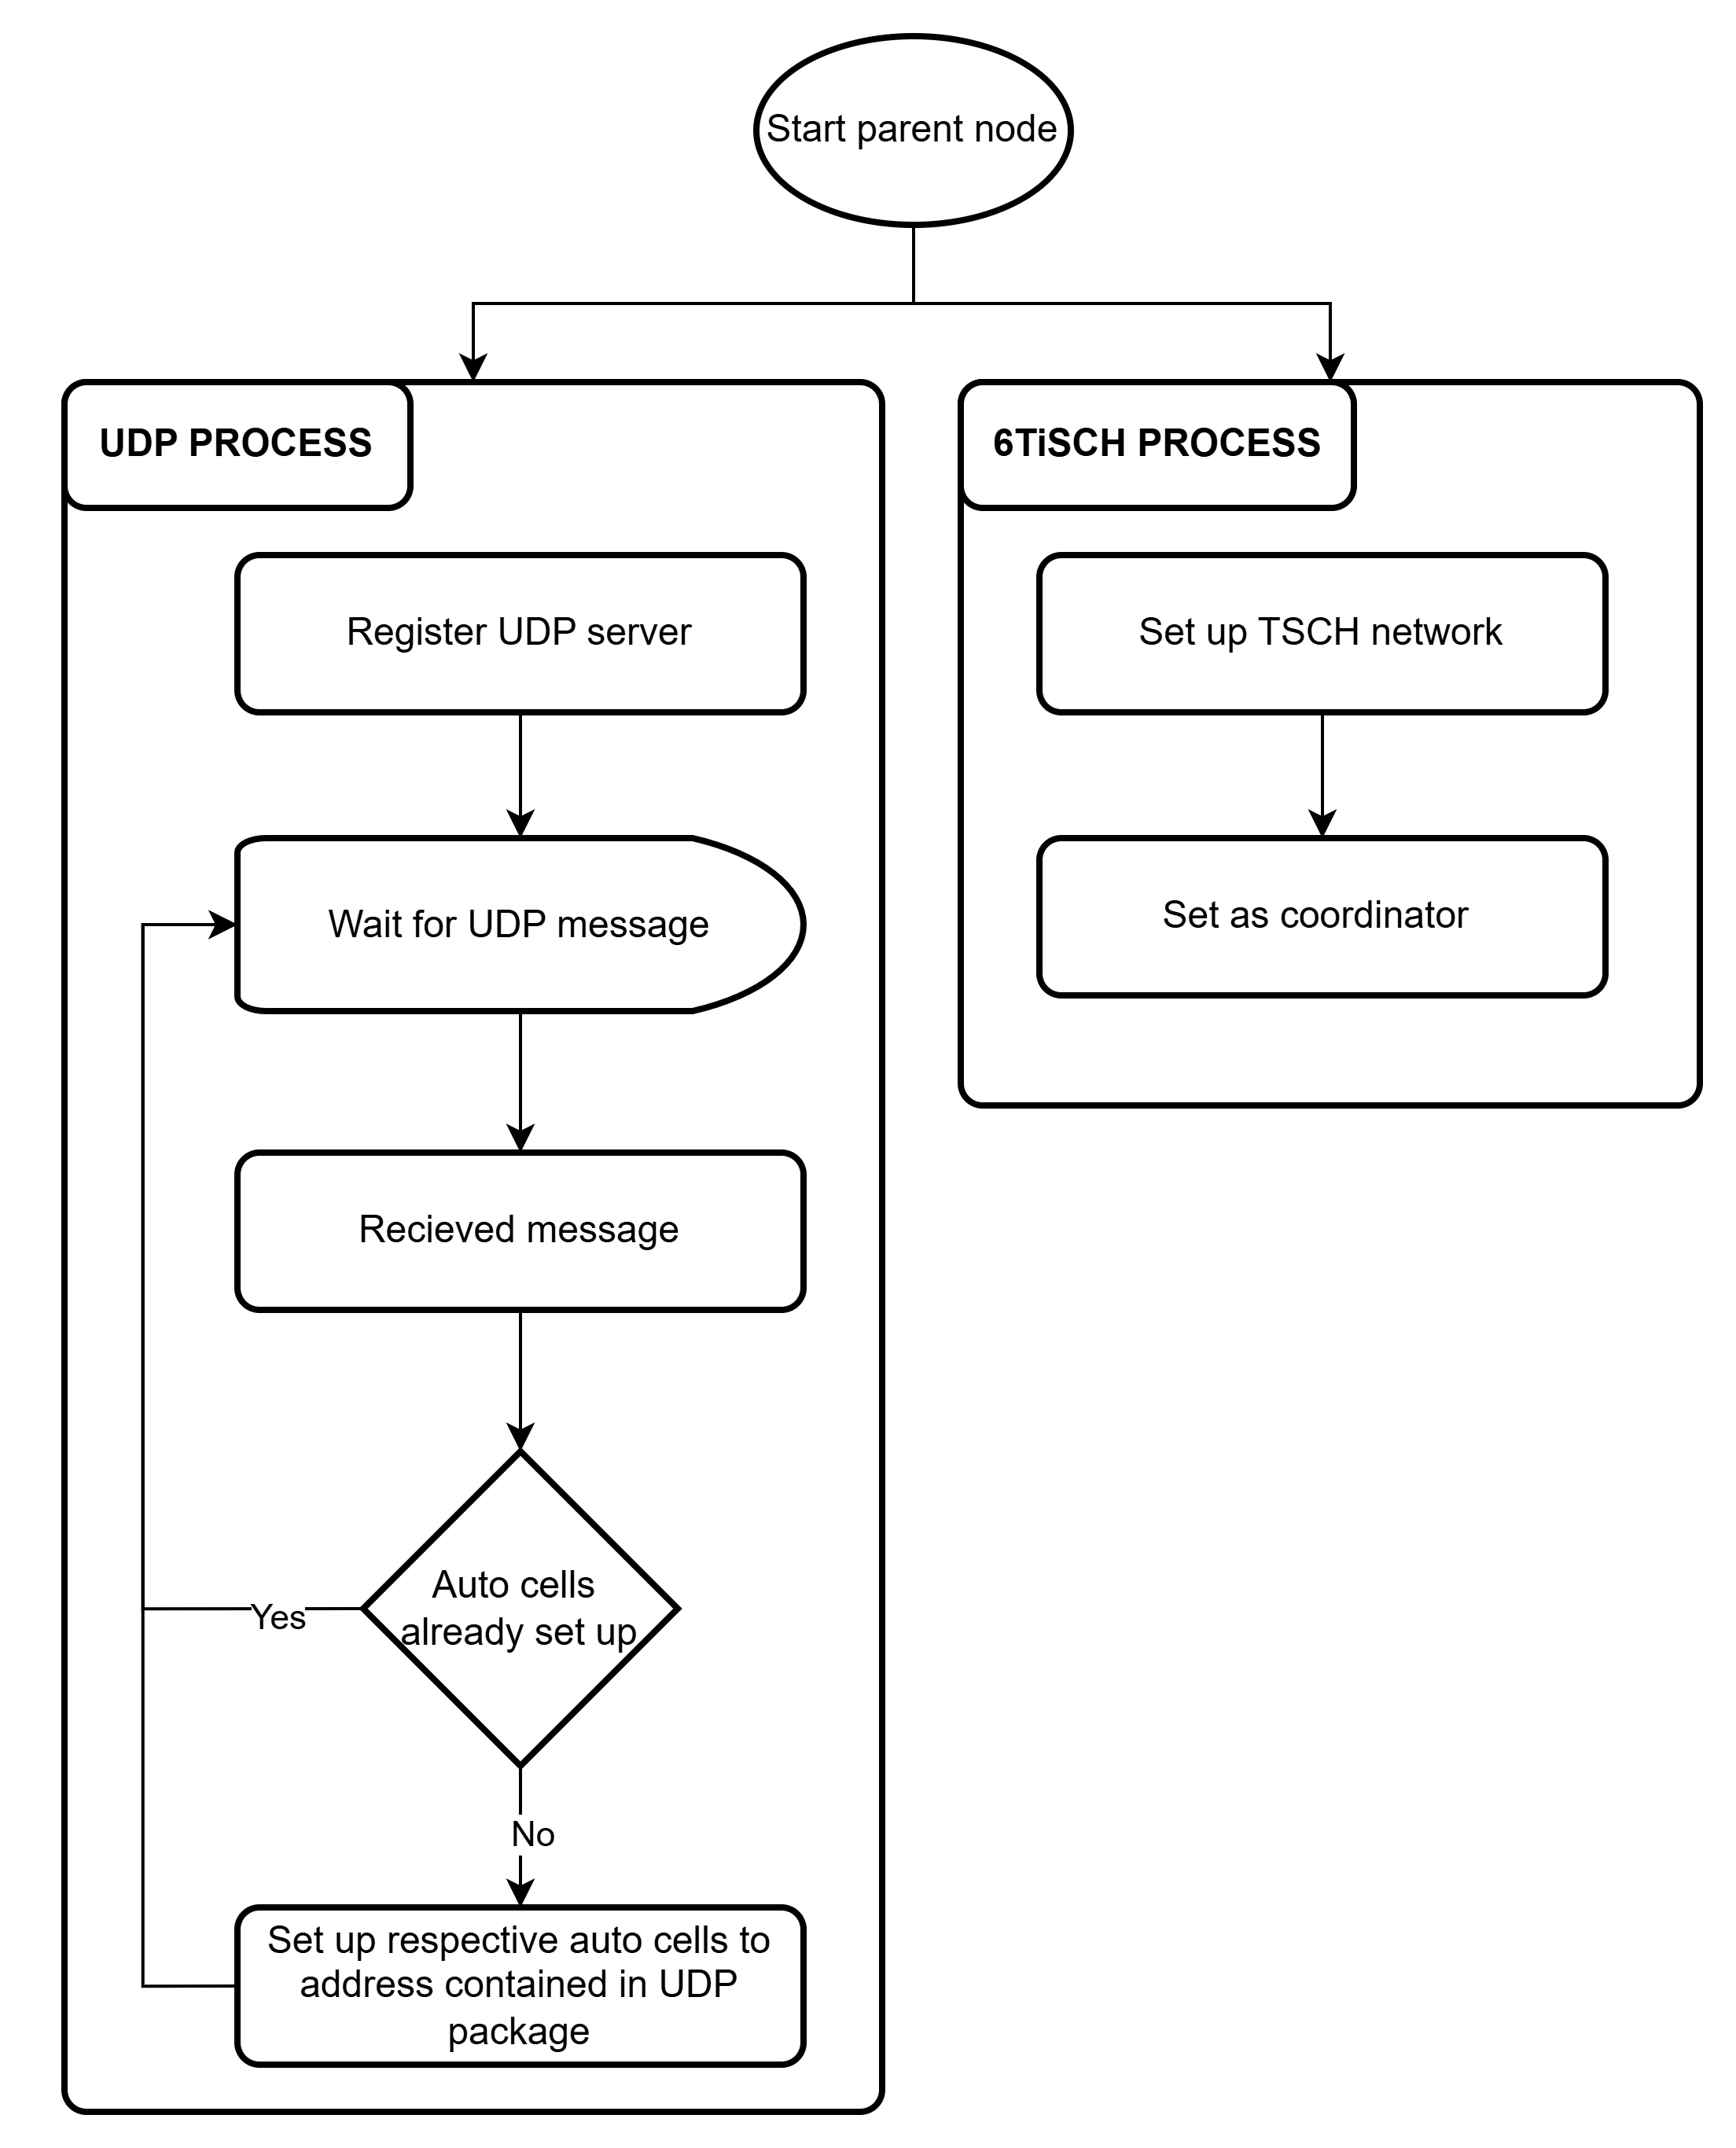
\includegraphics[width=0.7\textwidth]{./images/parent-node-flowchart.png}
    \caption{Flowchart of parent nodes actions.}
    \label{fig:parent-node-flowchart}
\end{figure}


\subsection*{Child Node}
The child node is the target node, which allocates cells for communication with the parent and, if there is interference, relocates the cells. To emulate the real life scenario as much as possible the child node also sends UDP packages to the parent with a an interval of

\begin{equation}
    t_{send} = \frac{CLOCK\_SECOND}{n_{tx}u_c} + t_{var}
\end{equation}

where $t_{send}$ is the time in clockticks between each package. It is computed taking $CLOCK\_SECOND$, which is a physical second in platform specific clockticks and dividing it by $n_{tx}$ the amount of currently allocated cells multiplied by $u_c$ which is the cell utilization factor. Finally $t_{var}$ as small variance variable is added at the end, to ensure all cells are used

All these three functionalities translate directly into their respective processes which are presented in Figure \ref{fig:child-node-flowchart}.
The UDP process is responsible for sending the UDP packets to the parent with the above mentioned frequency.
The \ac{6P} add process first initializes \ac{TSCH} and joins the network. Upon successful joining of the node to the network the process adds the autonomous cells to the parent and logs the time of the start of the experiment. Then cell additions take place till the the target amount of cells per slotframe is reached where it then terminates. The time until MAX\_NUM\_CELLS have elapsed is estimated by dividing MAX\_NUM\_CELLS by $n_{tx}$ and multiplying that with the slotframe length in seconds.
At last the \ac{6P} relocate process waits for the node to fully join the network and then evaluates each HOUSEKEEPINGCOLLISION\_PERIOD whether relocations are necessary. In case relocations are necessary the node compiles a list of cells that need to be relocated then sends a relocation request for each cell.

\begin{figure}[H]
    \centering
    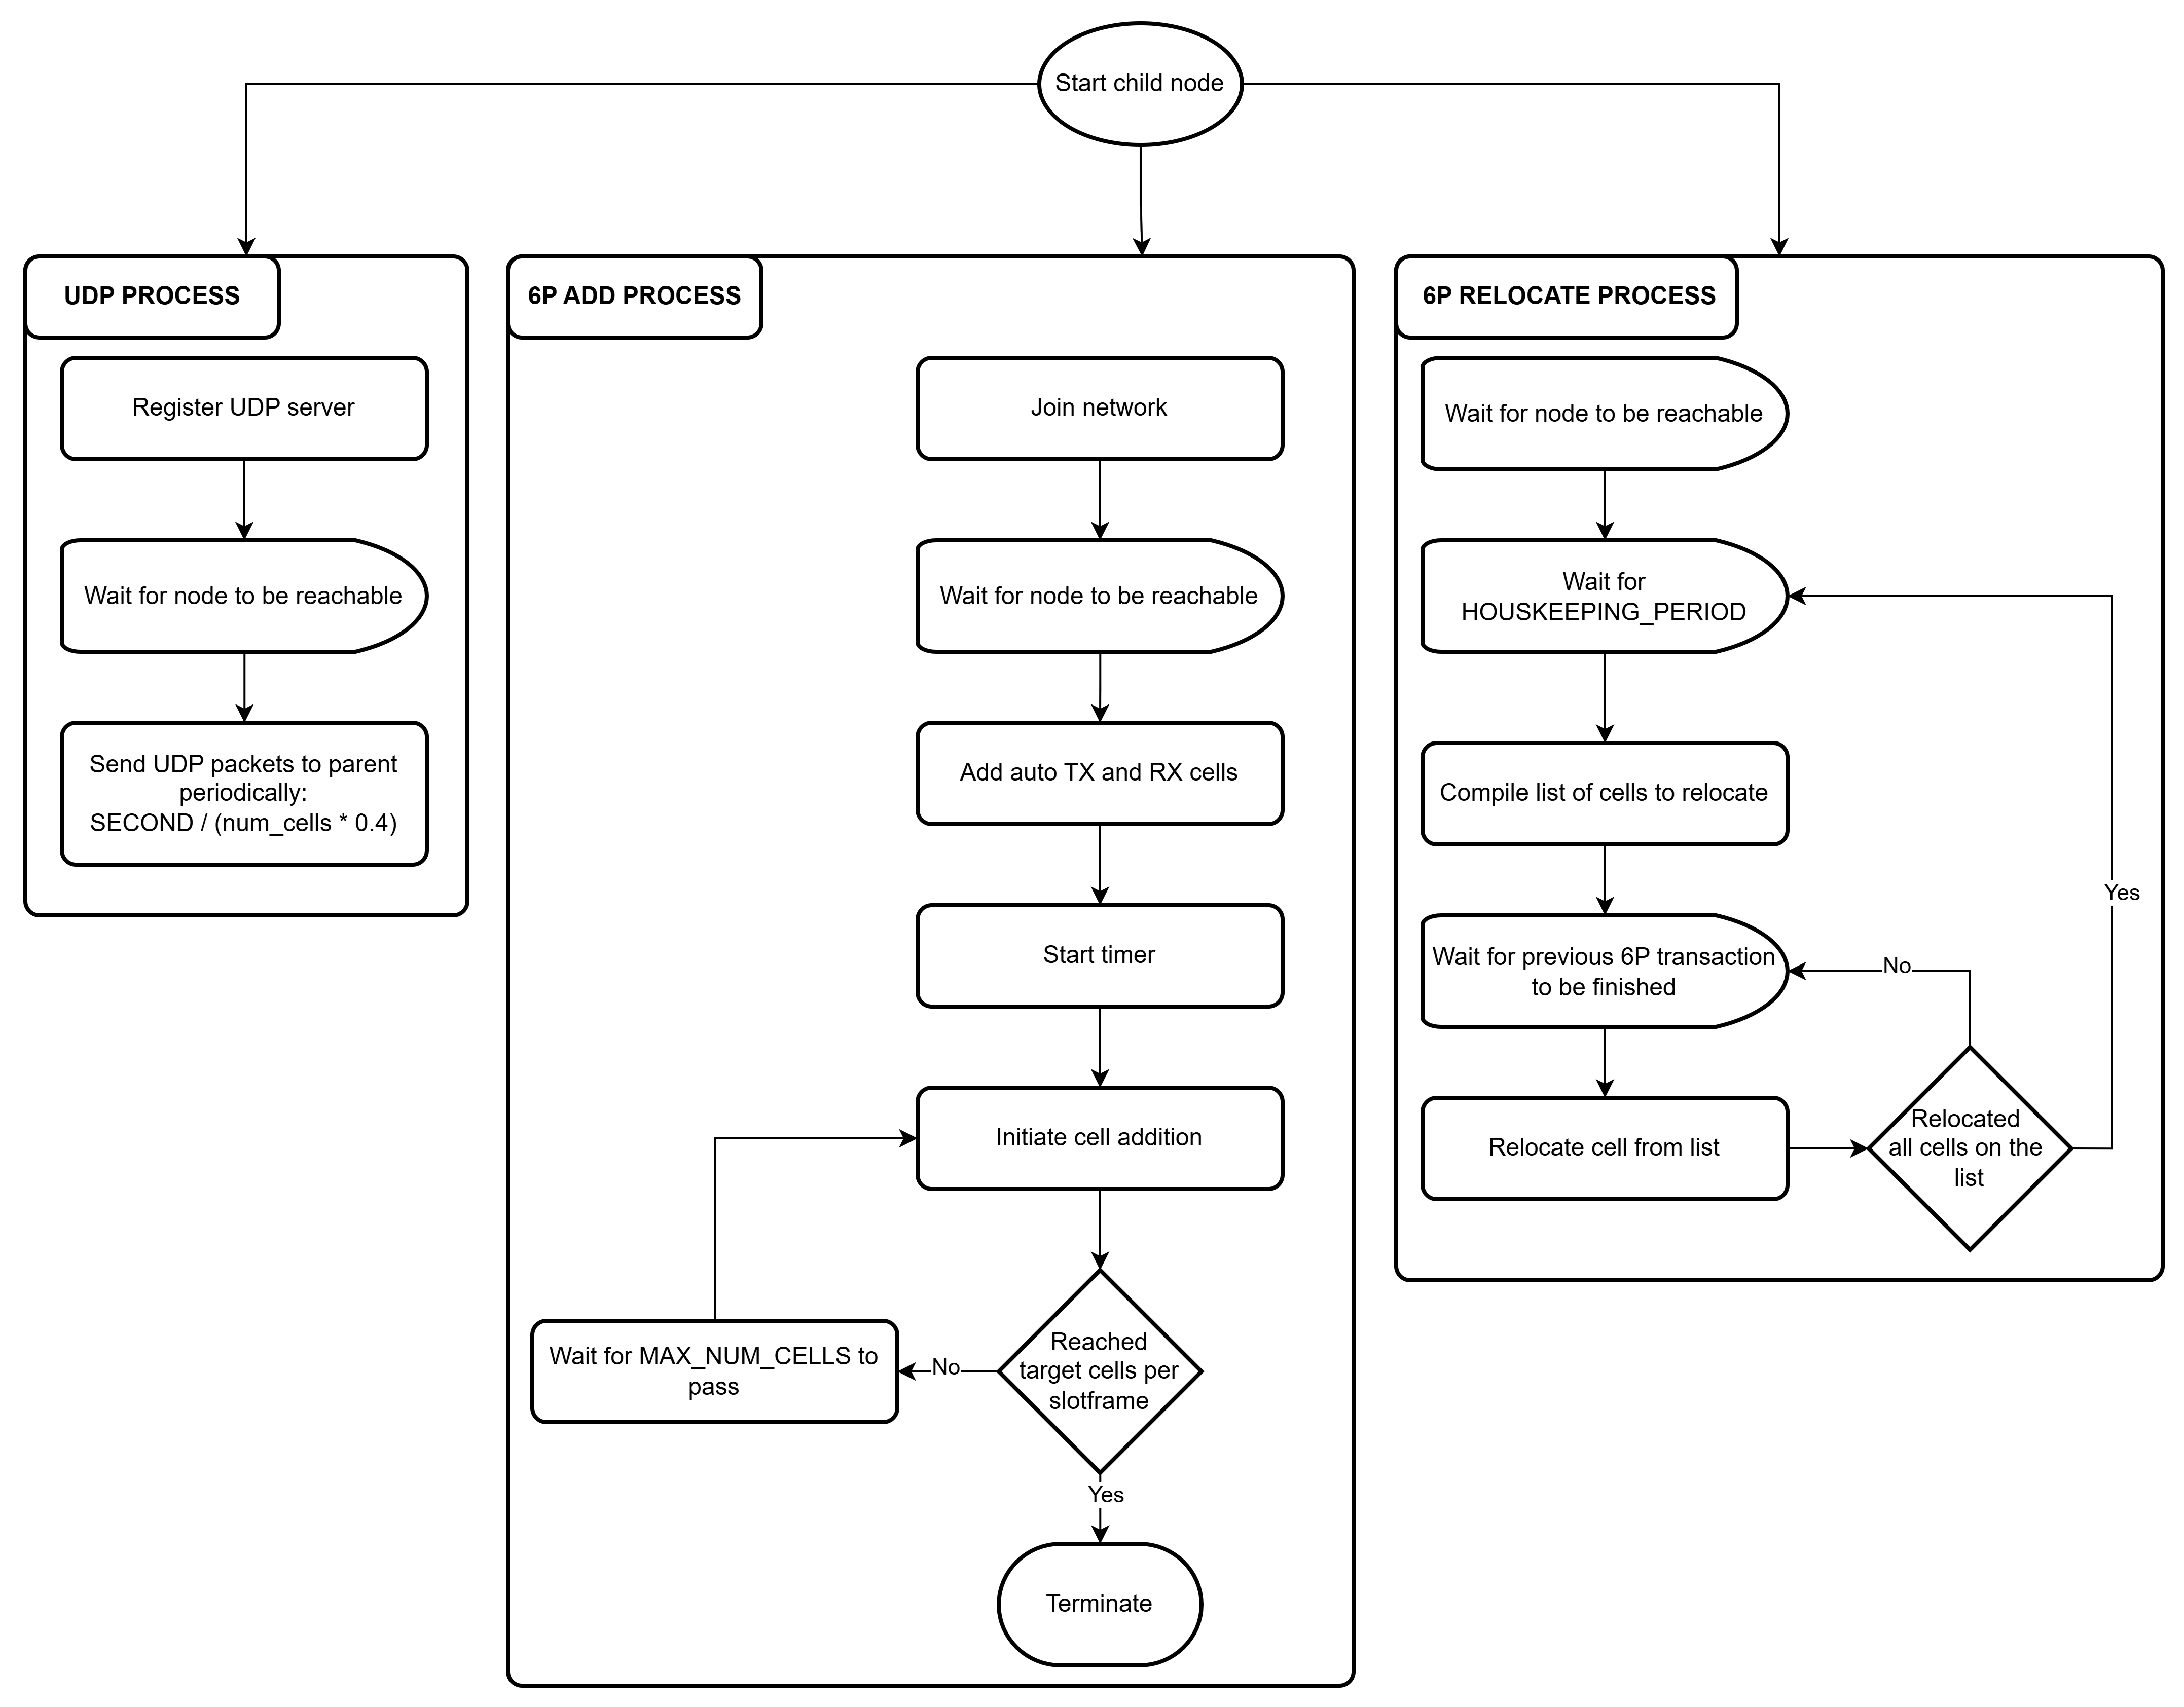
\includegraphics[width=1\textwidth]{./images/child-node-flowchart.png}
    \caption{Flowchart of child nodes actions.}
    \label{fig:child-node-flowchart}
\end{figure}

\subsection*{Network Node}
The network node has the function to act as the emulator for the rest of the \ac{6TiSCH} network with a constant traffic load N packets per slotframe. To achieve that the cell initialization process of the node first joins the network and then randomly generates a given num\_cells\_interfere amount of cells to be allocated for interference. Once the node has joined the network these cells are added to the schedule manually, meaning without negotiating and sending \ac{6P} requests and upon adding all cells, the process terminates.
To interfere on the allocated cells the UDP process first sets up a \ac{UDP} server and upon successfully joining the network autonomous Tx cells to the parent are allocated to enure stable communication for \ac{RPL} and \ac{TSCH} control traffic. If interference is set to false then the node sends a \ac{UDP} package every second in order to allow the child node to successfully join the network without interfering with that too much, since the bootstrapping period of the network is not of interest for this research. Once the child node is connected to the network the parent will send a \ac{UDP} package to the network node informing it to start interferen upon which the node will start interfering with a periodicity of num\_cells\_interfere packets per second. These packets are \ac{UDP} broadcast with the nodes link layer address as payload.

\begin{figure}[H]
    \centering
    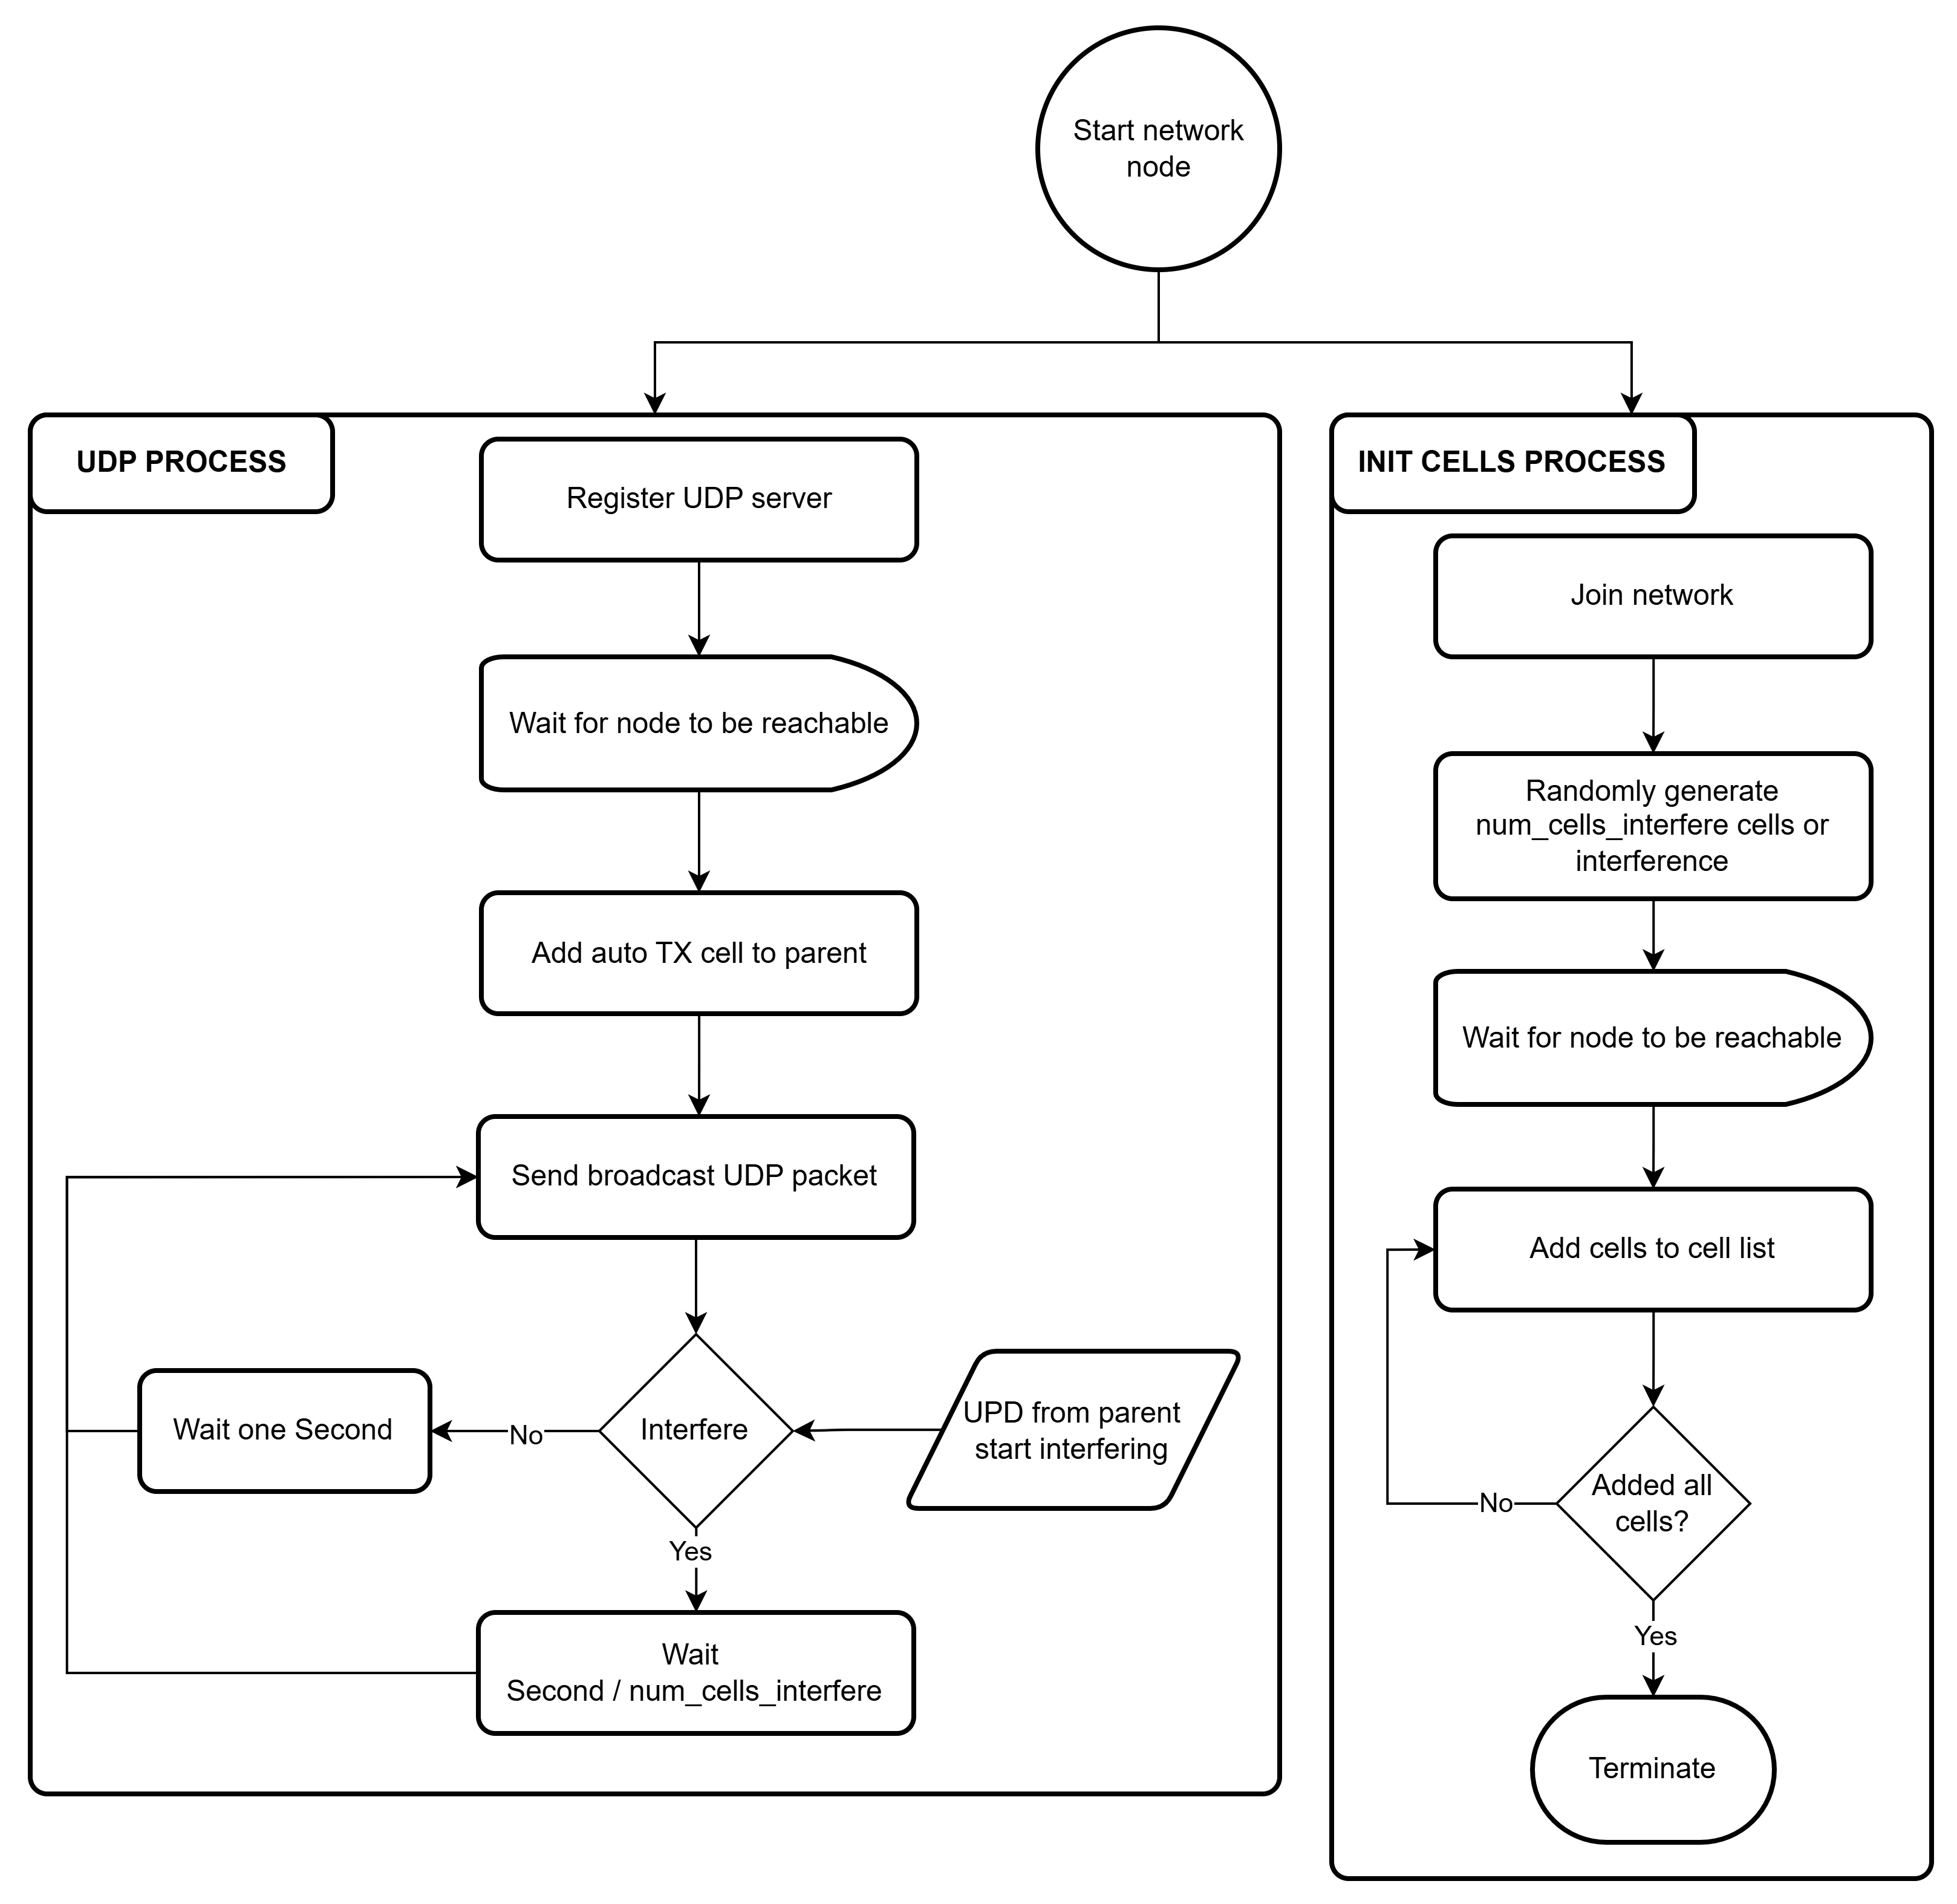
\includegraphics[width=1\textwidth]{./images/network-node-flowchart.png}
    \caption{Flowchart of network nodes actions.}
    \label{fig:network-node-flowchart}
\end{figure}


\subsection*{Additional Implementations}
\label{sec:add-implementations}
Since the simple \ac{SF} provided by the sixtop example only has cell additions and deletions, a relocation process needed to be implemented. For the \ac{SF} to be able to decide whether a relocation is necessary or not, it needs to have a precise information for every cell how many packets were sent, and how many of them were successful. The \ac{TSCH} API only supports the evaluation of whole channels meaning that only the performance of a channel was recorded and could be queried. That's why an additional mechanism was added which everytime a package is sent will keep a record of which cell it was sent on and whether it was successful or not. This was the relocation process can accurately calculate the \ac{PDR} of each cell and decide whether a cell needs to be relocated or not.
The relocation mechanism is designed similarly to the add and delete process. First all the entries of the cells are evaluated and the \ac{PDR} is calculated. Upon discovering a \ac{PDR} that is below the threshold a random candidate cell list is generated, which then together with the cell that is to be relocated and some metadata is inserted into a \ac{6P} relocated package and then sent via the \ac{6top} output API.
Receiving this \ac{6P} relocate request the parent node evaluates the candidate cell list and picks the first that is available. It then sends a \ac{6P} response with the chosen cell, allocates that cell and deletes the cell that is relocated from its schedule.
At last after receiving the \ac{6P} request the child also adds the chosen cell and deletes the relocated cell.


The sensing mechanism was implemented using a candidate list and a blacklist. In addition to that a randomly pre-generated list of cells was defined as cells in which the network node would interfere. Using these three lists the sensing mechanims would check before each cell allocation whether the cells in the candidate list were on the interference list. This implementation was chosen in order to emulate the sensing since the implementation of the sensing cells is not viable for the timeframe given.



\section{ Results and Discussion }
This section, based on the experimental setup and application design explained before presents the results of the experiment and compares them with the results of the analytical model proposed in section \ref{chp:model}. For this comparison two \acp{KPI} are taken into account namely the scheduling time, which is the time it takes for the schedule to reach a stable state $T_s$ and the probability of a cell that is allocated to overlap with an occupied cell $p_ov$. The common parameters of the experiments are presented in Table \ref{tab:common-para-ex}. In total 8 experiments were conducted with each 10 runs allocating 25 cells in one run with 4 using the default cell allocation mechanism and 4 the sensing mechanism. For each i-th cell $T_s$ was tracked, recorded and logged in the end of the experiment enabling us to have $T_s$, $T_a$ values and the amount of relocations for $\mu_{\max}$ from 2-25 cells. The results presented are the average of all the runs with a confidence interval of 95\%. 
The network interference is evaluated on 20\% and 10\% due to the limitations of using only one node as emulator for the network, since physically it at most can only send on one cell each timeslot and experimentally it turned out that a higher load leads to inconsistency in the nodes performance. 

\begin{table}[h]
    \centering
    \caption{Common parameters of all experiments.}
    \begin{tabular}{|c|c|}
    \hline
    MAX\_NUMTX & 32 \\ \hline
    HOUSEKEEPINGCOLLISION\_PERIOD & 60s  \\ \hline
    NUM\_CH\_OFFSET & 4 \\ \hline
    SLOTFRAME\_LENGTH & 101 slots  \\ \hline
    RELOCATE\_PDRTHRES & 50\%  \\ \hline
    Number of runs & 10  \\ \hline
    \end{tabular}
    \label{tab:common-para-ex}
\end{table}

\subsection*{Scheduling time}
First we consider the scheduling time, since it is a effective \ac{KPI} in determining the performance of the cell allocation mechanism, because it reflects both efficiency and and quality of the cell allocation mechanism. It is to be noted, that for the experimental approach we measured the point in time where no allocation was made whereas the analytical model gives the time the last relocation was done. In order to accout for this discrepancy one an subtract one HOUSEKEEPINGCOLLISION\_PERIOD from the experimental results. 
For the first experiment the following parameters were used.

\begin{table}[h]
    \centering
    \caption{Paramters for the first experiment.}
    \begin{tabular}{|c|c|}
    \hline
    MAX\_NUM\_CELLS & 100 \\ \hline
    Network interference N & 20\%  \\ \hline
    \end{tabular}
\end{table}

\begin{figure}[H]
    \centering
    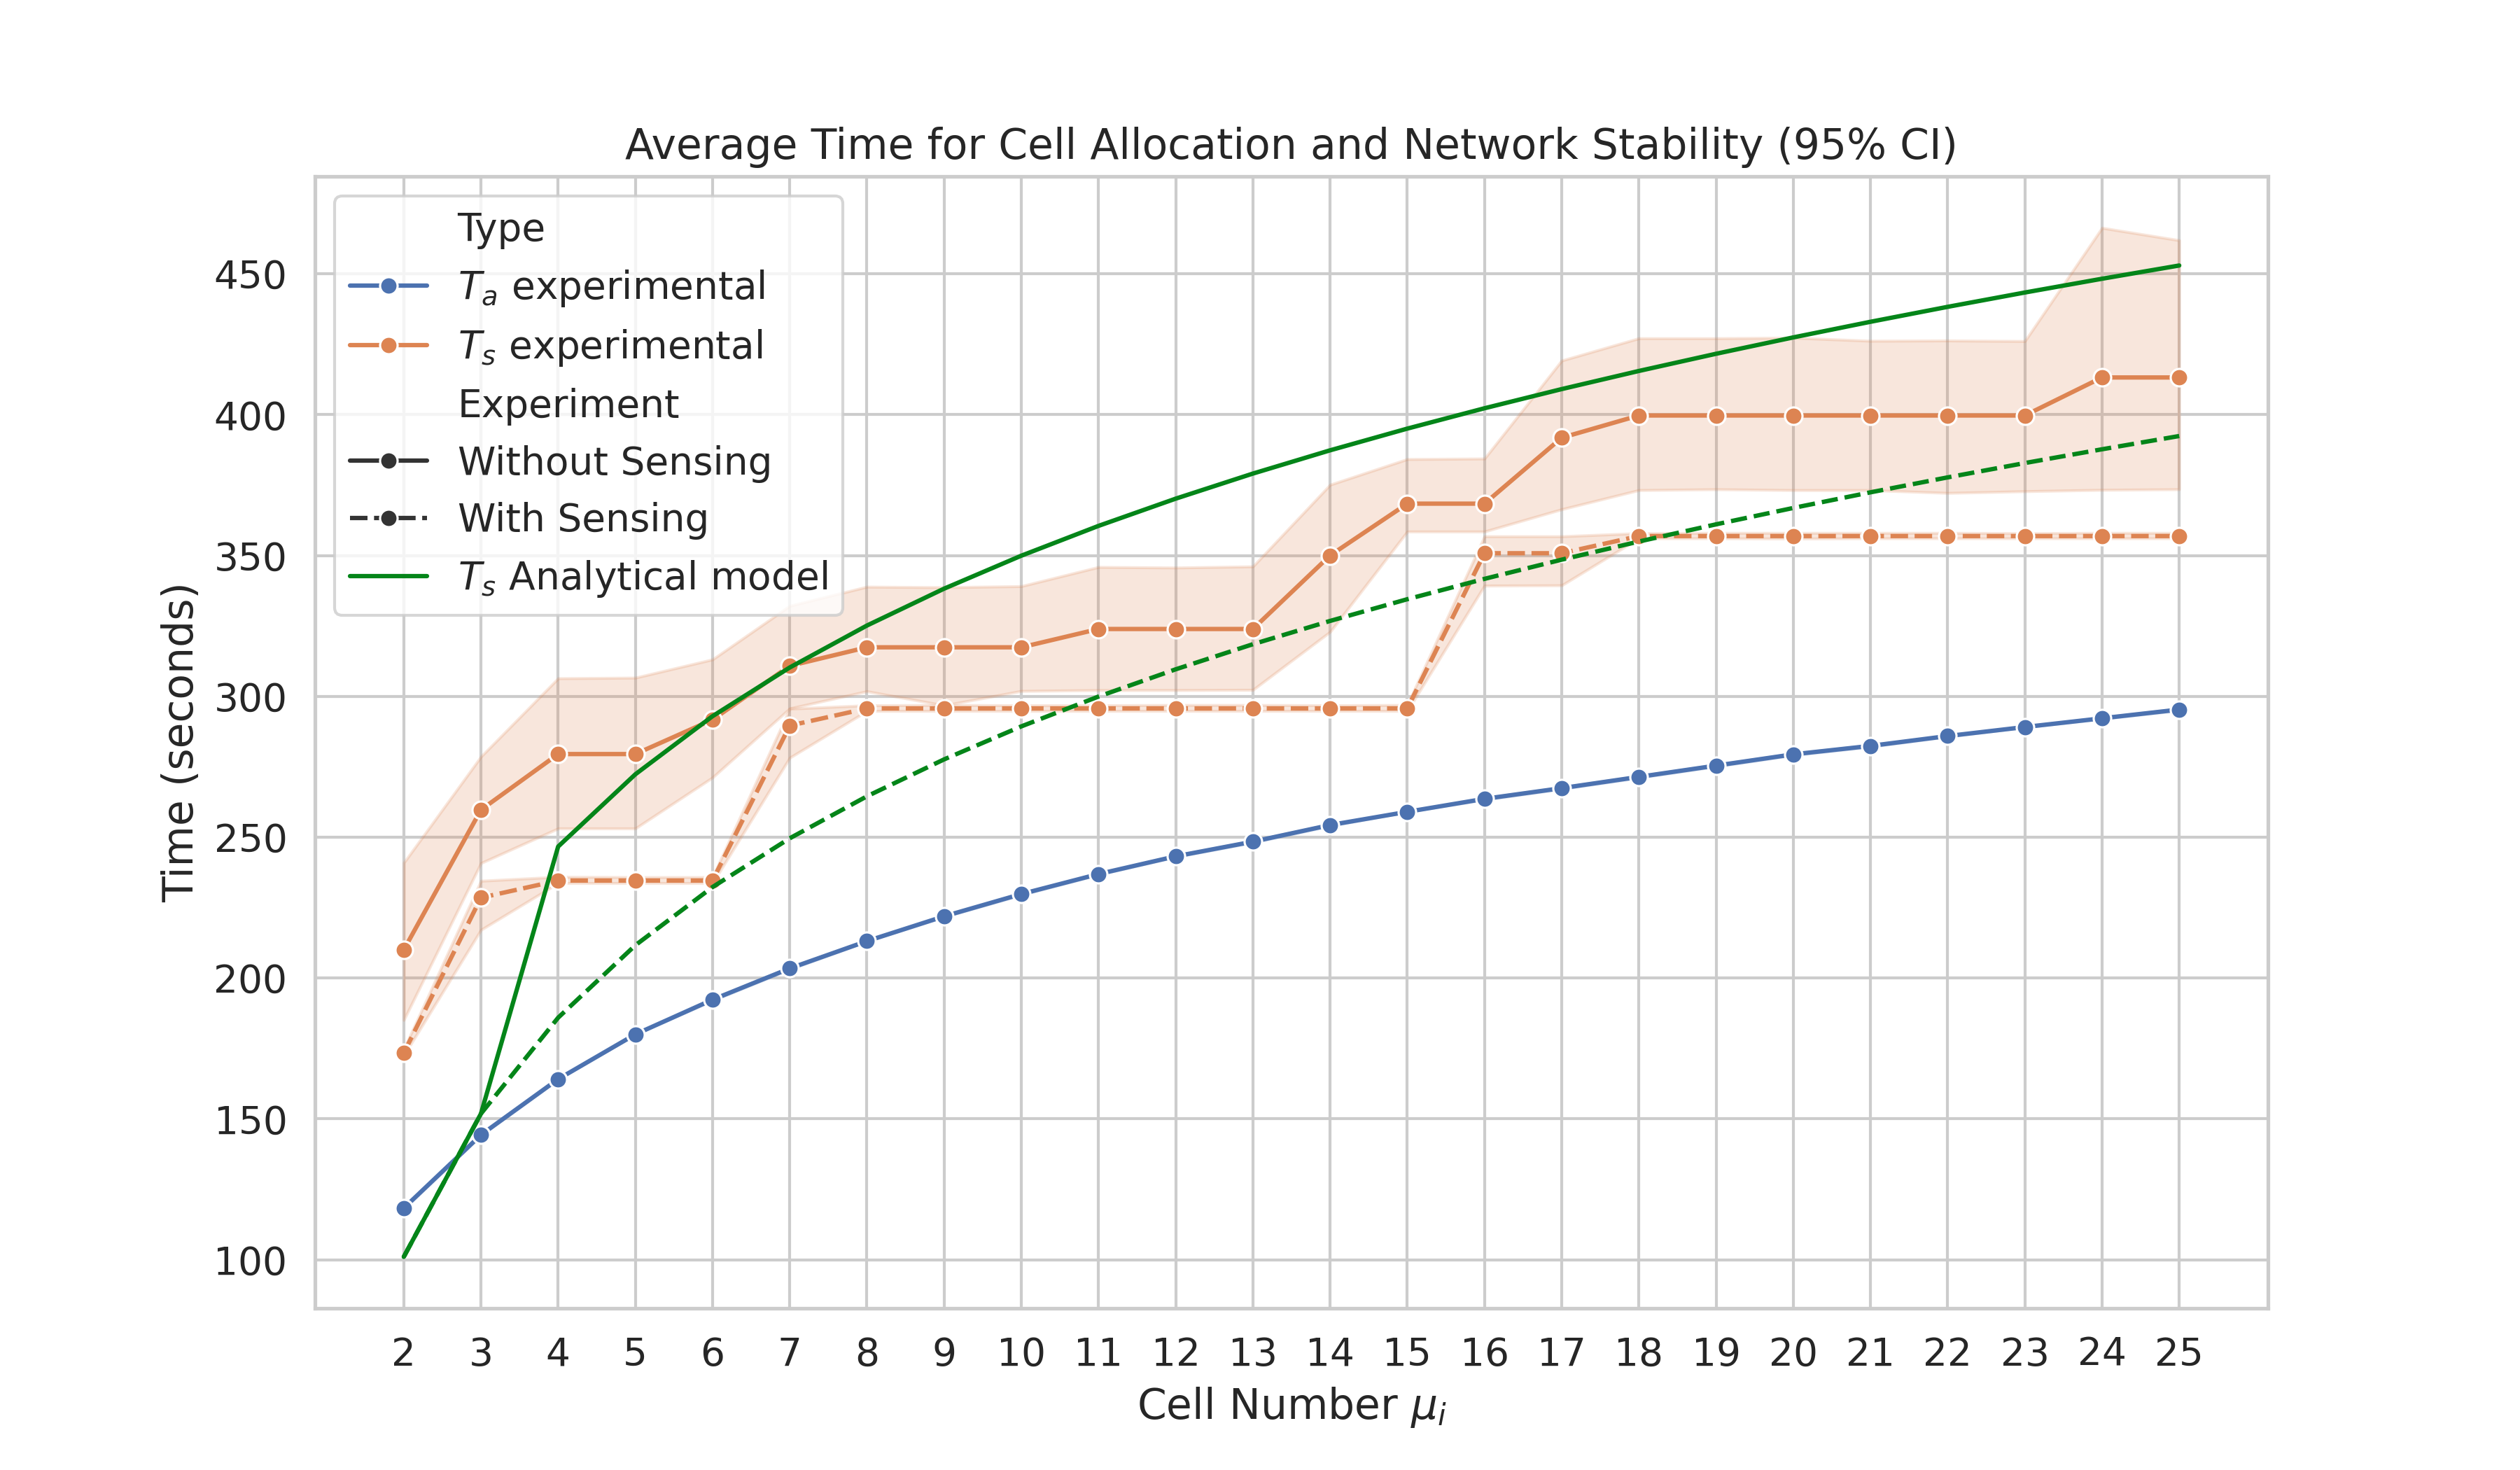
\includegraphics[width=1\textwidth]{./images/experiment1.png}
    \caption{Experimental and analytical results with medium interference.}
    \label{fig:experiment-1}
\end{figure}

Using the recommended value for MAX\_NUM\_CELLS and a network interference of 20\% i.e. 80 cells interfered out of 400 total available cells Figure \ref{fig:experiment-1} plots the experimental results with the expected analytical outcomes.
For the $T_a$ obtained from the experiment we can observe that with increasing $\mu_{\max}$ the time it takes to allocate an additional cell decreases since MAX\_NUM\_CELLS is reached faster leading to a shorter time until another cell is added. Since the implementation uses a timer to estimate the time it takes for MAX\_NUM\_CELLS to be reached by NumCellsElapsed and the fact that the variation of \ac{6P} add requests is minuscule the result is a smooth but slowing increase in time it takes to allocate the cells.
Considering $T_s$ the sensing mechanism consistently outperforms the non sensing mechanism as predicted by the analytical model presented in Equation \ref{eq:t_s}. The experiments roughly match the shape and values of the analytical model while only differing significantly in their sudden increases. The stepwise increase of the experimental data is due to the fact that if another relocation is needed it takes another HOUSEKEEPINGCOLLISION\_PERIOD to relocate again and the smooth graph for the analytical data is because it works with averaged values.
The variance of the non sensing mechanism is notably higher than the sensing mechanims since the sensing mechanism has next to no overlap leading to at most one relocation whereas the amount of relocation periods necessary for the non sensing mechanism can vary highly. The reason for that is for instance the fact, that the time it takes to register a cell as having a \ac{PDR} that is too low can vary since even if the cell is interfered with it might not be in every slotframe, so some messages do get sent successfully.

To study the allocation mechanism under different network interference loads the second experiment had a network interference of 10\%.

\begin{figure}[H]
    \centering
    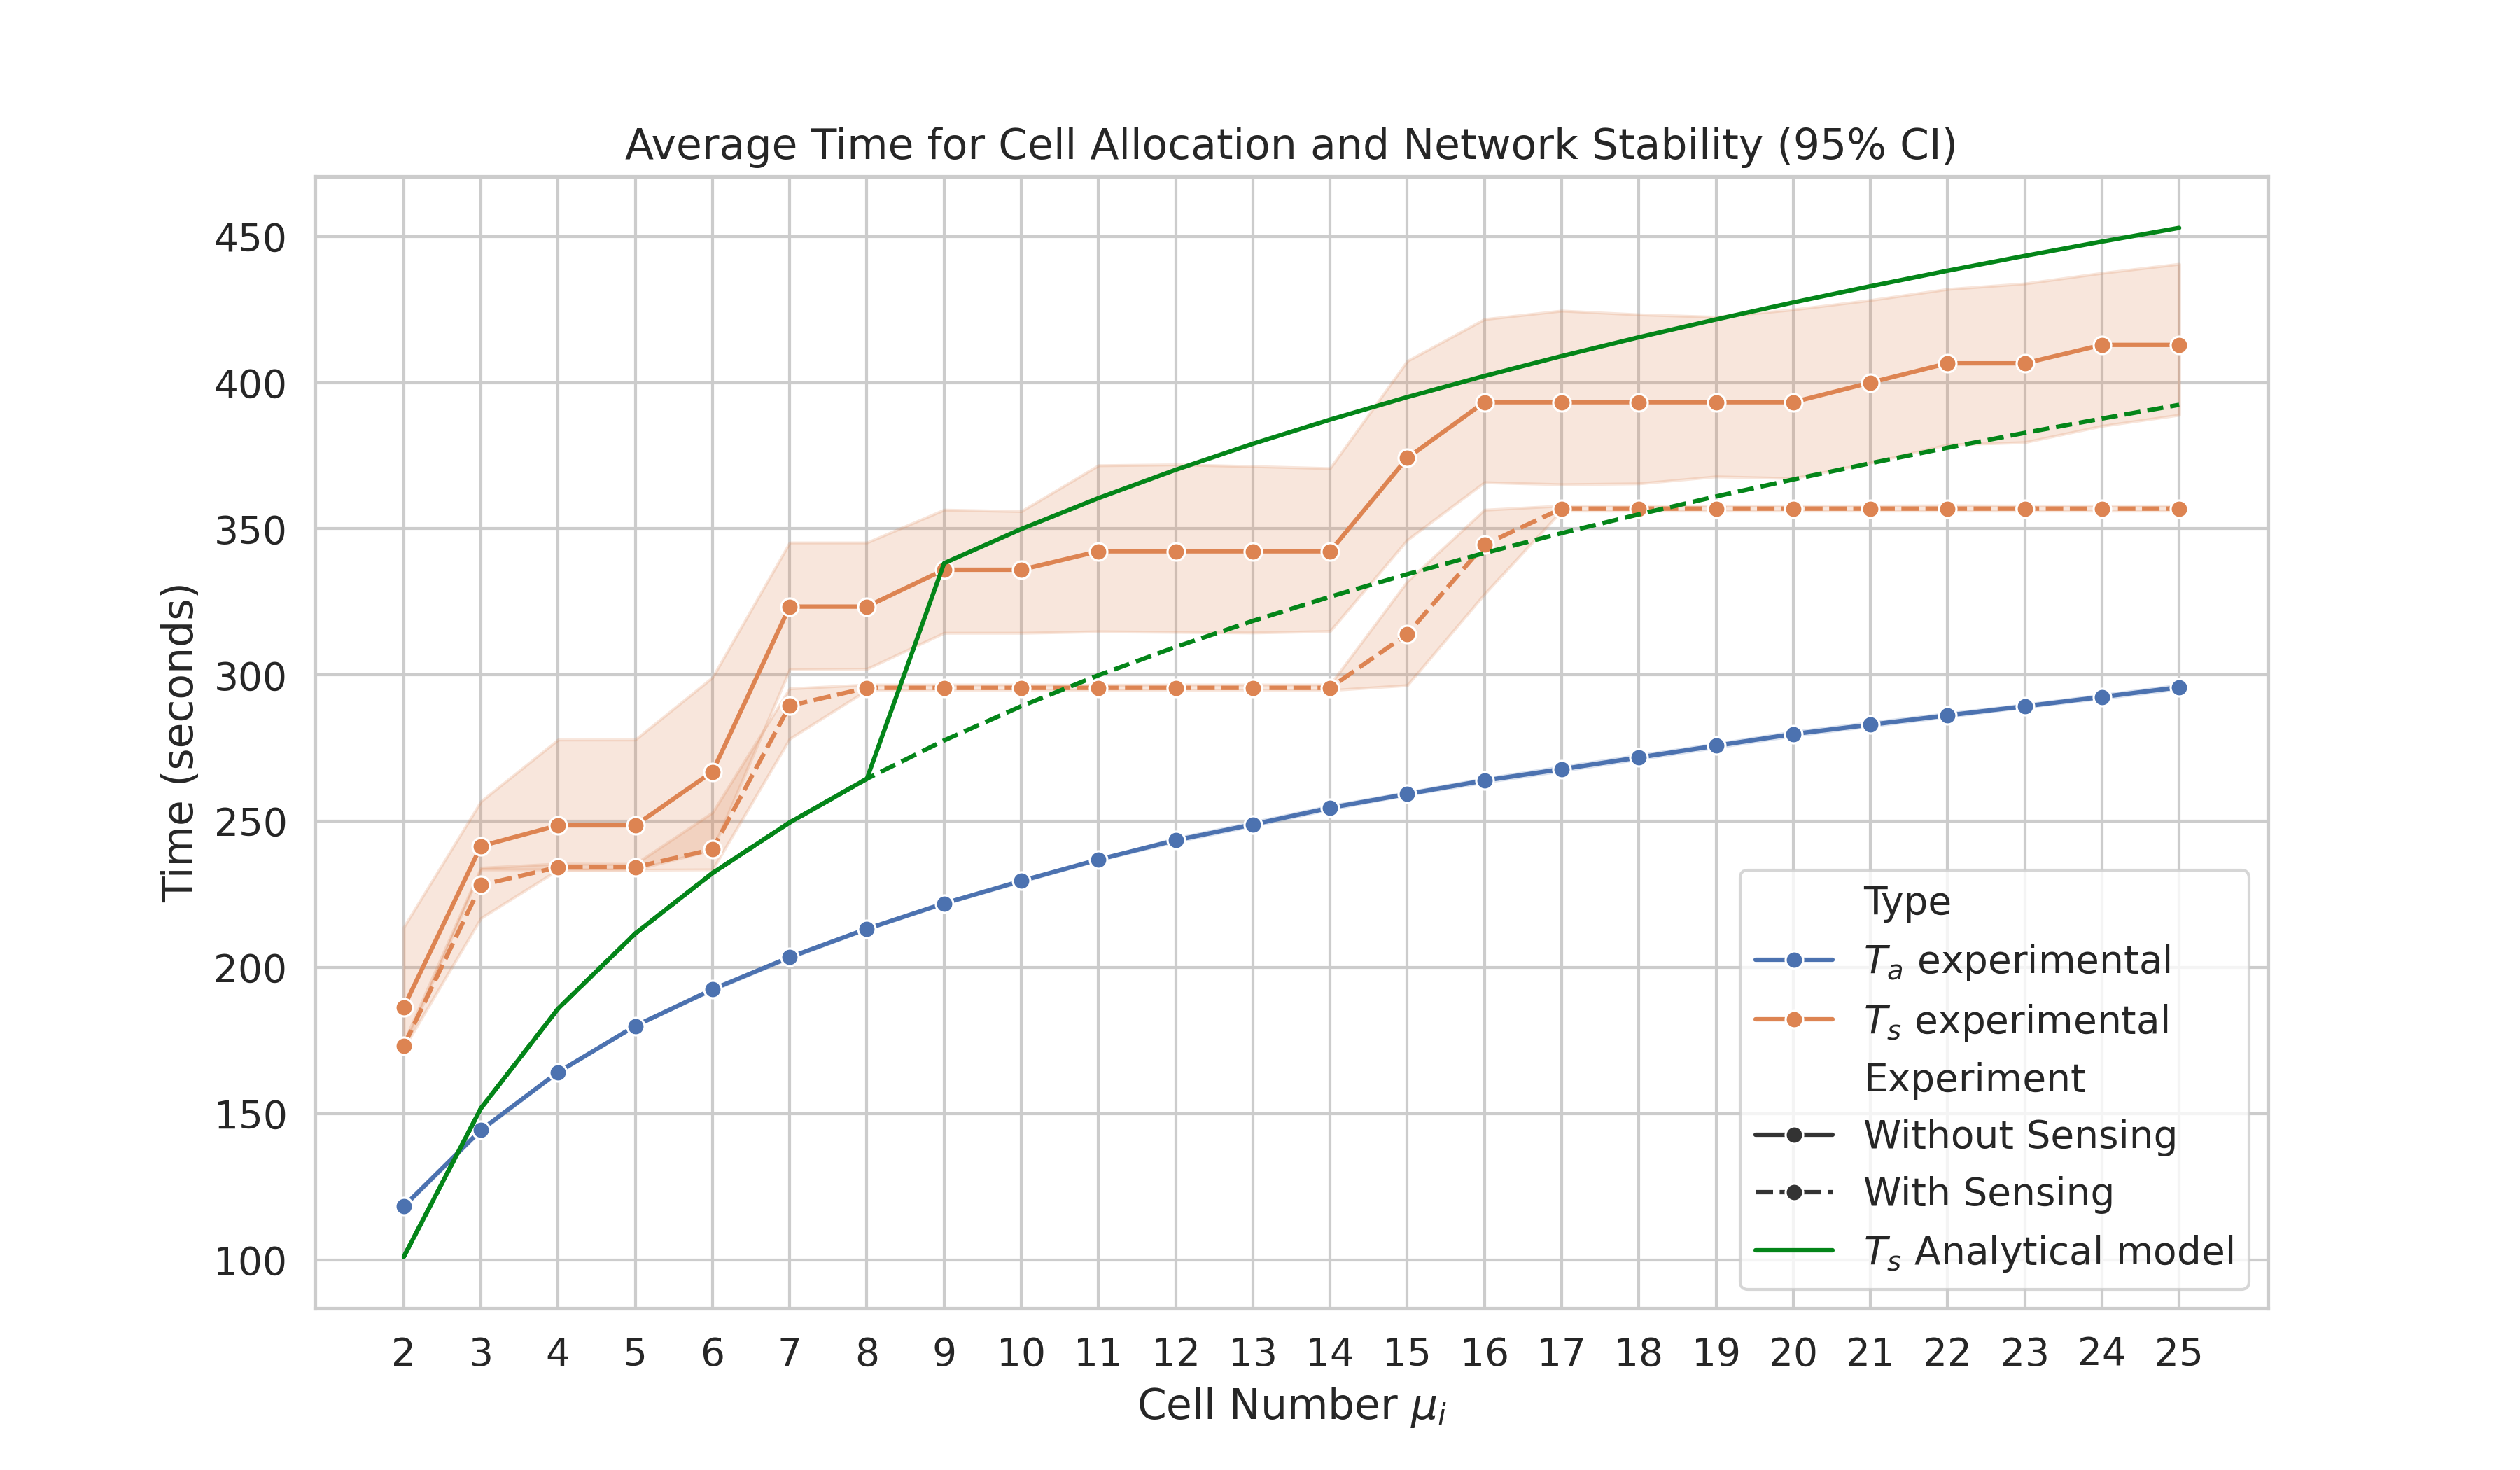
\includegraphics[width=1\textwidth]{./images/experiment2.png}
    \caption{Experimental and analytical results with 10\% network interference.}
    \label{fig:experiment-2}
\end{figure}

Similarly to the first experiment the sensing mechanism consistently outperforms the non sensing mechanism and both align with the analytical expectations. Overall compared to an interference of 20\% $T_a$ remains unchanged and $T_s$ only is slightly lower to about a $\mu_{\max}$ of 7 for the experimental and 8 for the analytical before it becomes very similar. This is because in the beginning the likelyhood of a relocation occuring at all very low, but the more cells are allocated the more it grows until it reached a point where at least one relocation must be done, where the amount of relocations then does not play that big of a role anymore. 
This is why with a lower interference the point where the sensing and non sensing mechanims diverge in terms of $T_s$ is later at 8 cells whereas for medium interference they already diverge at 3 cells. The probability of overlap starts lower and increases slower, making the non sensing mechanism behave closer to the sensing one for longer.


In addition to varying the network interference we also varied the \ac{MSF} parameter MAX\_NUM\_CELLS to study the effect of faster cell allocation on the cell allocation process.

\begin{table}[h]
    \centering
    \caption{Paramters for the third experiment.}
    \begin{tabular}{|c|c|}
    \hline
    MAX\_NUM\_CELLS & 50 \\ \hline
    Network interference N & 20\%  \\ \hline
    \end{tabular}
\end{table}

\begin{figure}[H]
    \centering
    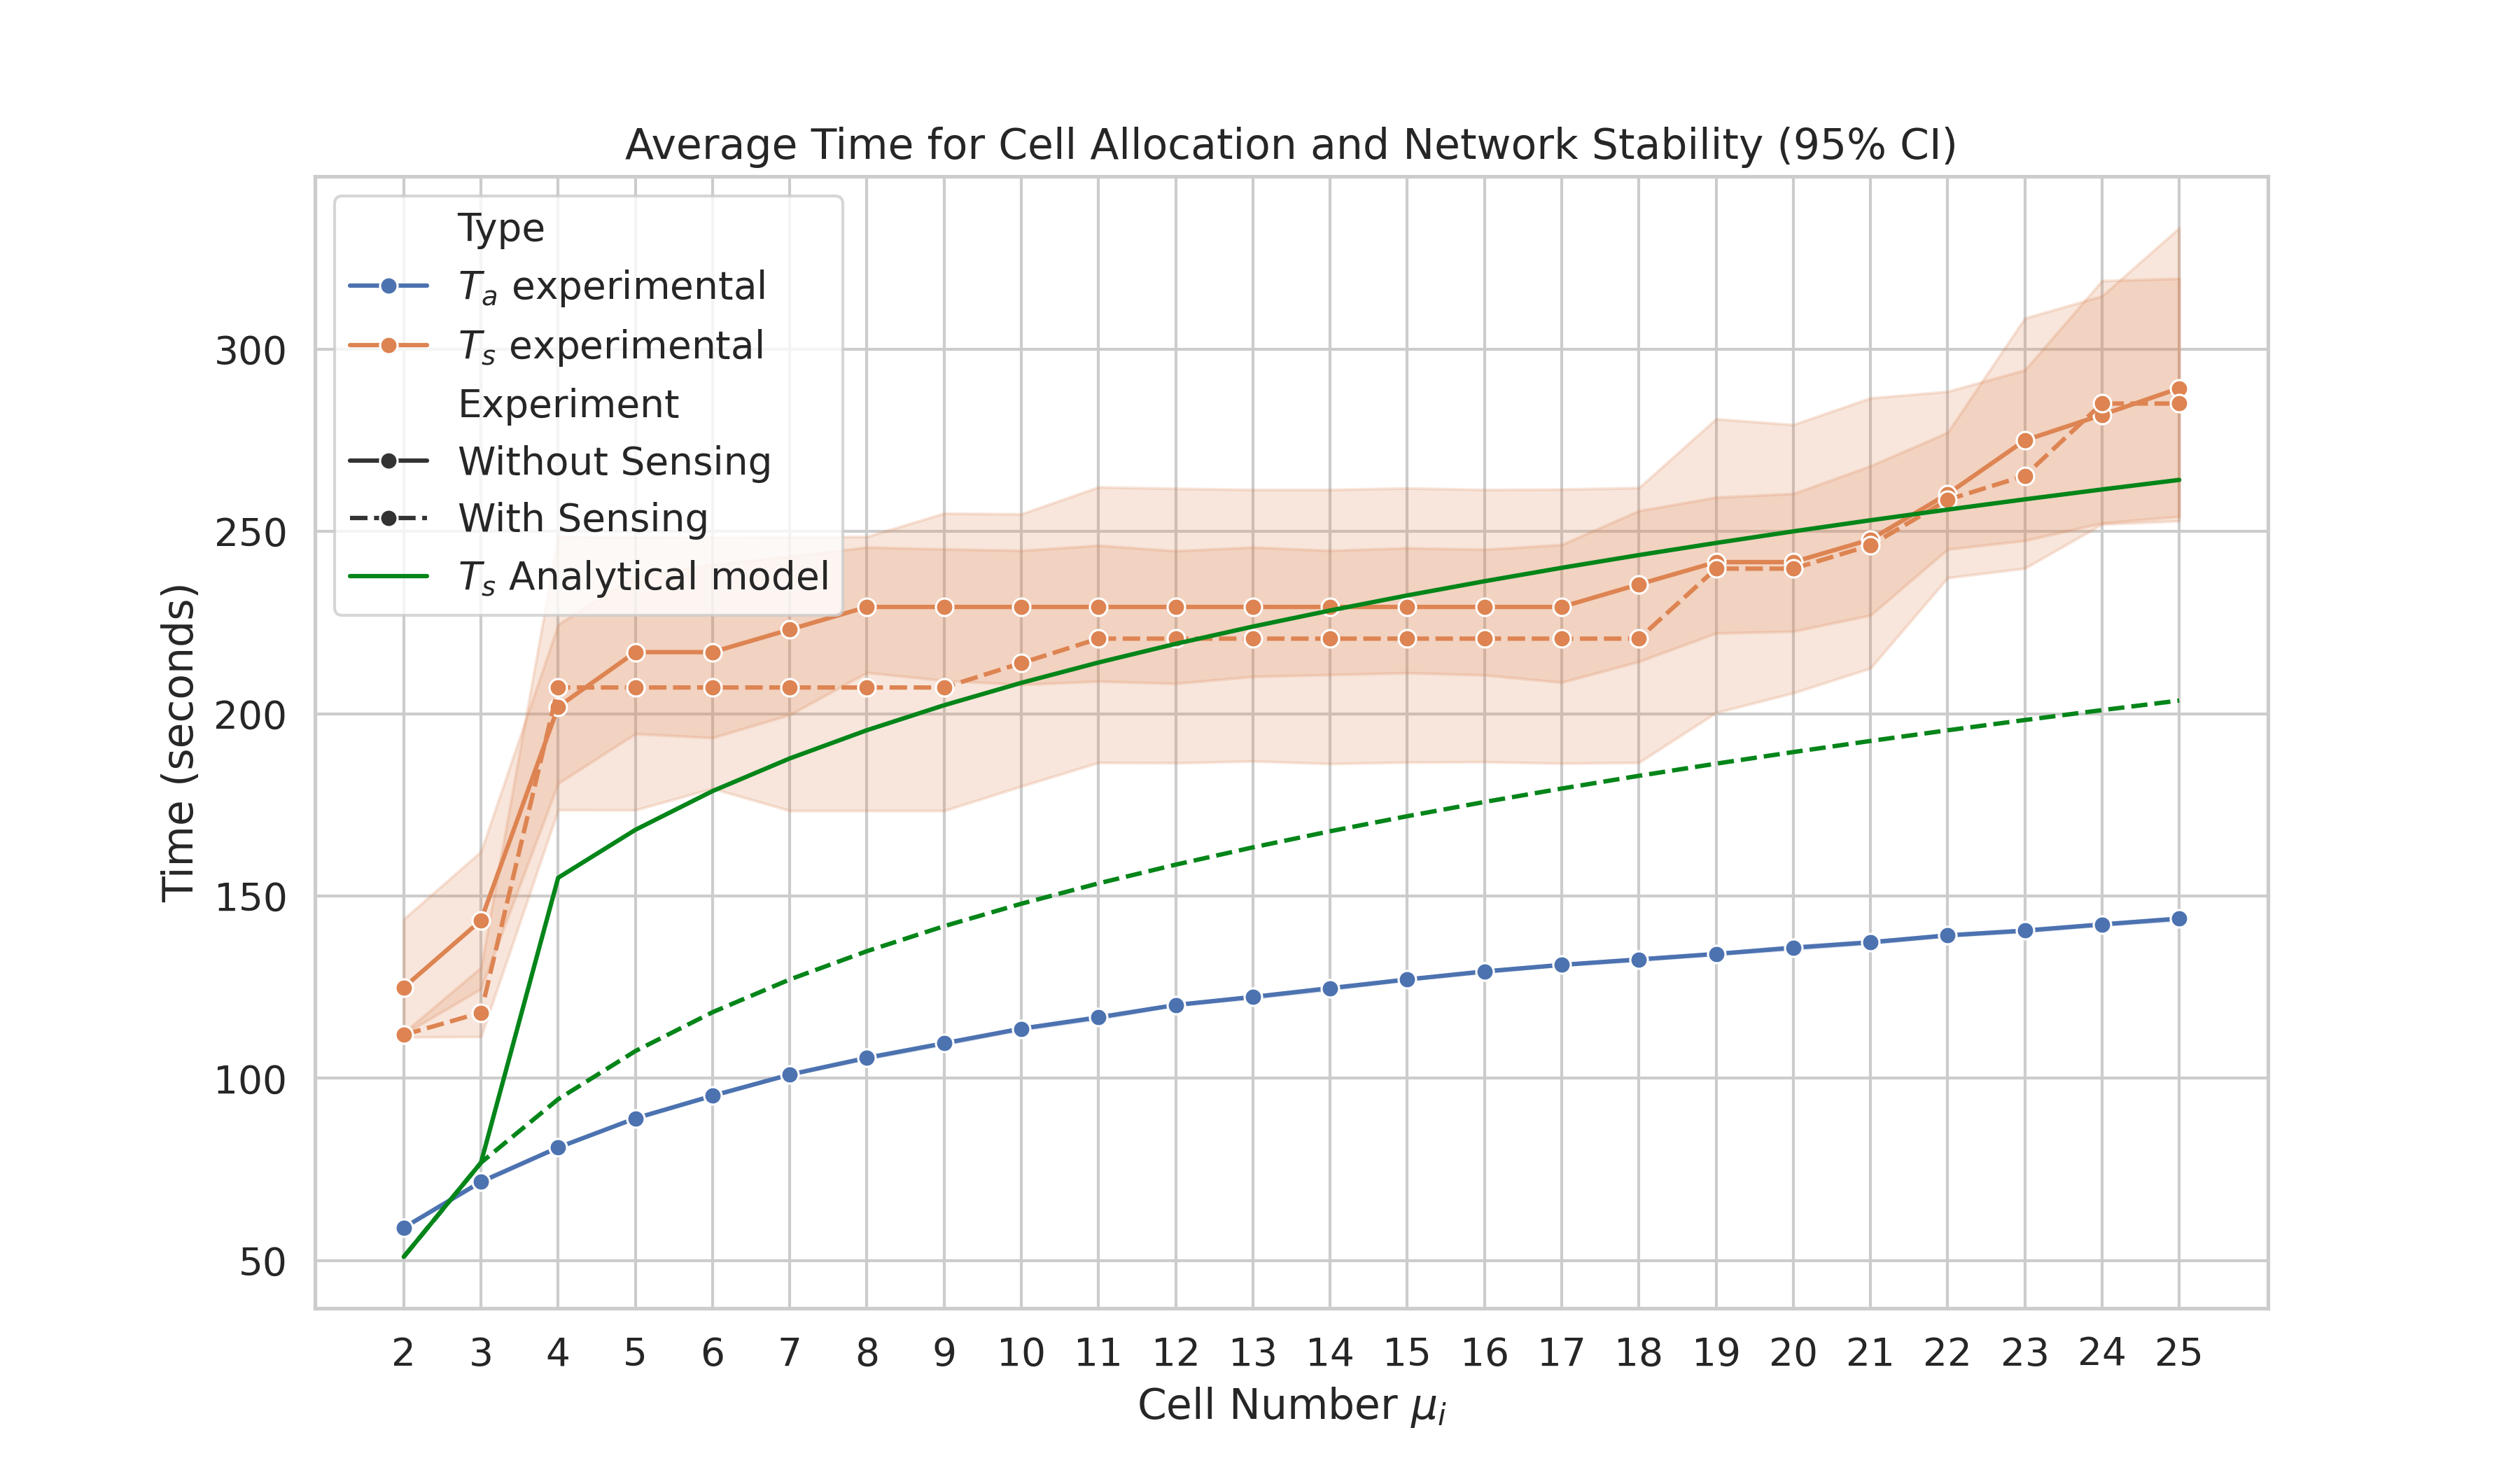
\includegraphics[width=1\textwidth]{./images/experiment3.png}
    \caption{Results of low MAX\_NUM\_CELLS with medium interference.}
    \label{fig:experiment-3}
\end{figure}

As expected $T_a$ significantly decreased from over 100 seconds with MAX\_NUM\_CELLS of 100 to about 60 second for MAX\_NUM\_CELLS of 50 in the second cell and this relationship is consistent for all cells. This is because it takes less time for NumCellsElapsed to reach MAX\_NUM\_CELLS leading to more frequent cell allocations. 
As for $T_s$ it also decreased by up to 100 seconds compared to before. Although the non sensing experimental values align well with the analytical expectations the values from the sensing mechanism are not as distinced from the non sensing mechanism as before. Due to experimental fluctuations with external interference?


At last we consider the network under low network interference with low MAX\_NUM\_CELLS.

\begin{table}[h]
    \centering
    \caption{Paramters for the fourth experiment.}
    \begin{tabular}{|c|c|}
    \hline
    MAX\_NUM\_CELLS & 50 \\ \hline
    Network interference N & 10\%  \\ \hline
    \end{tabular}
\end{table}

\begin{figure}[H]
    \centering
    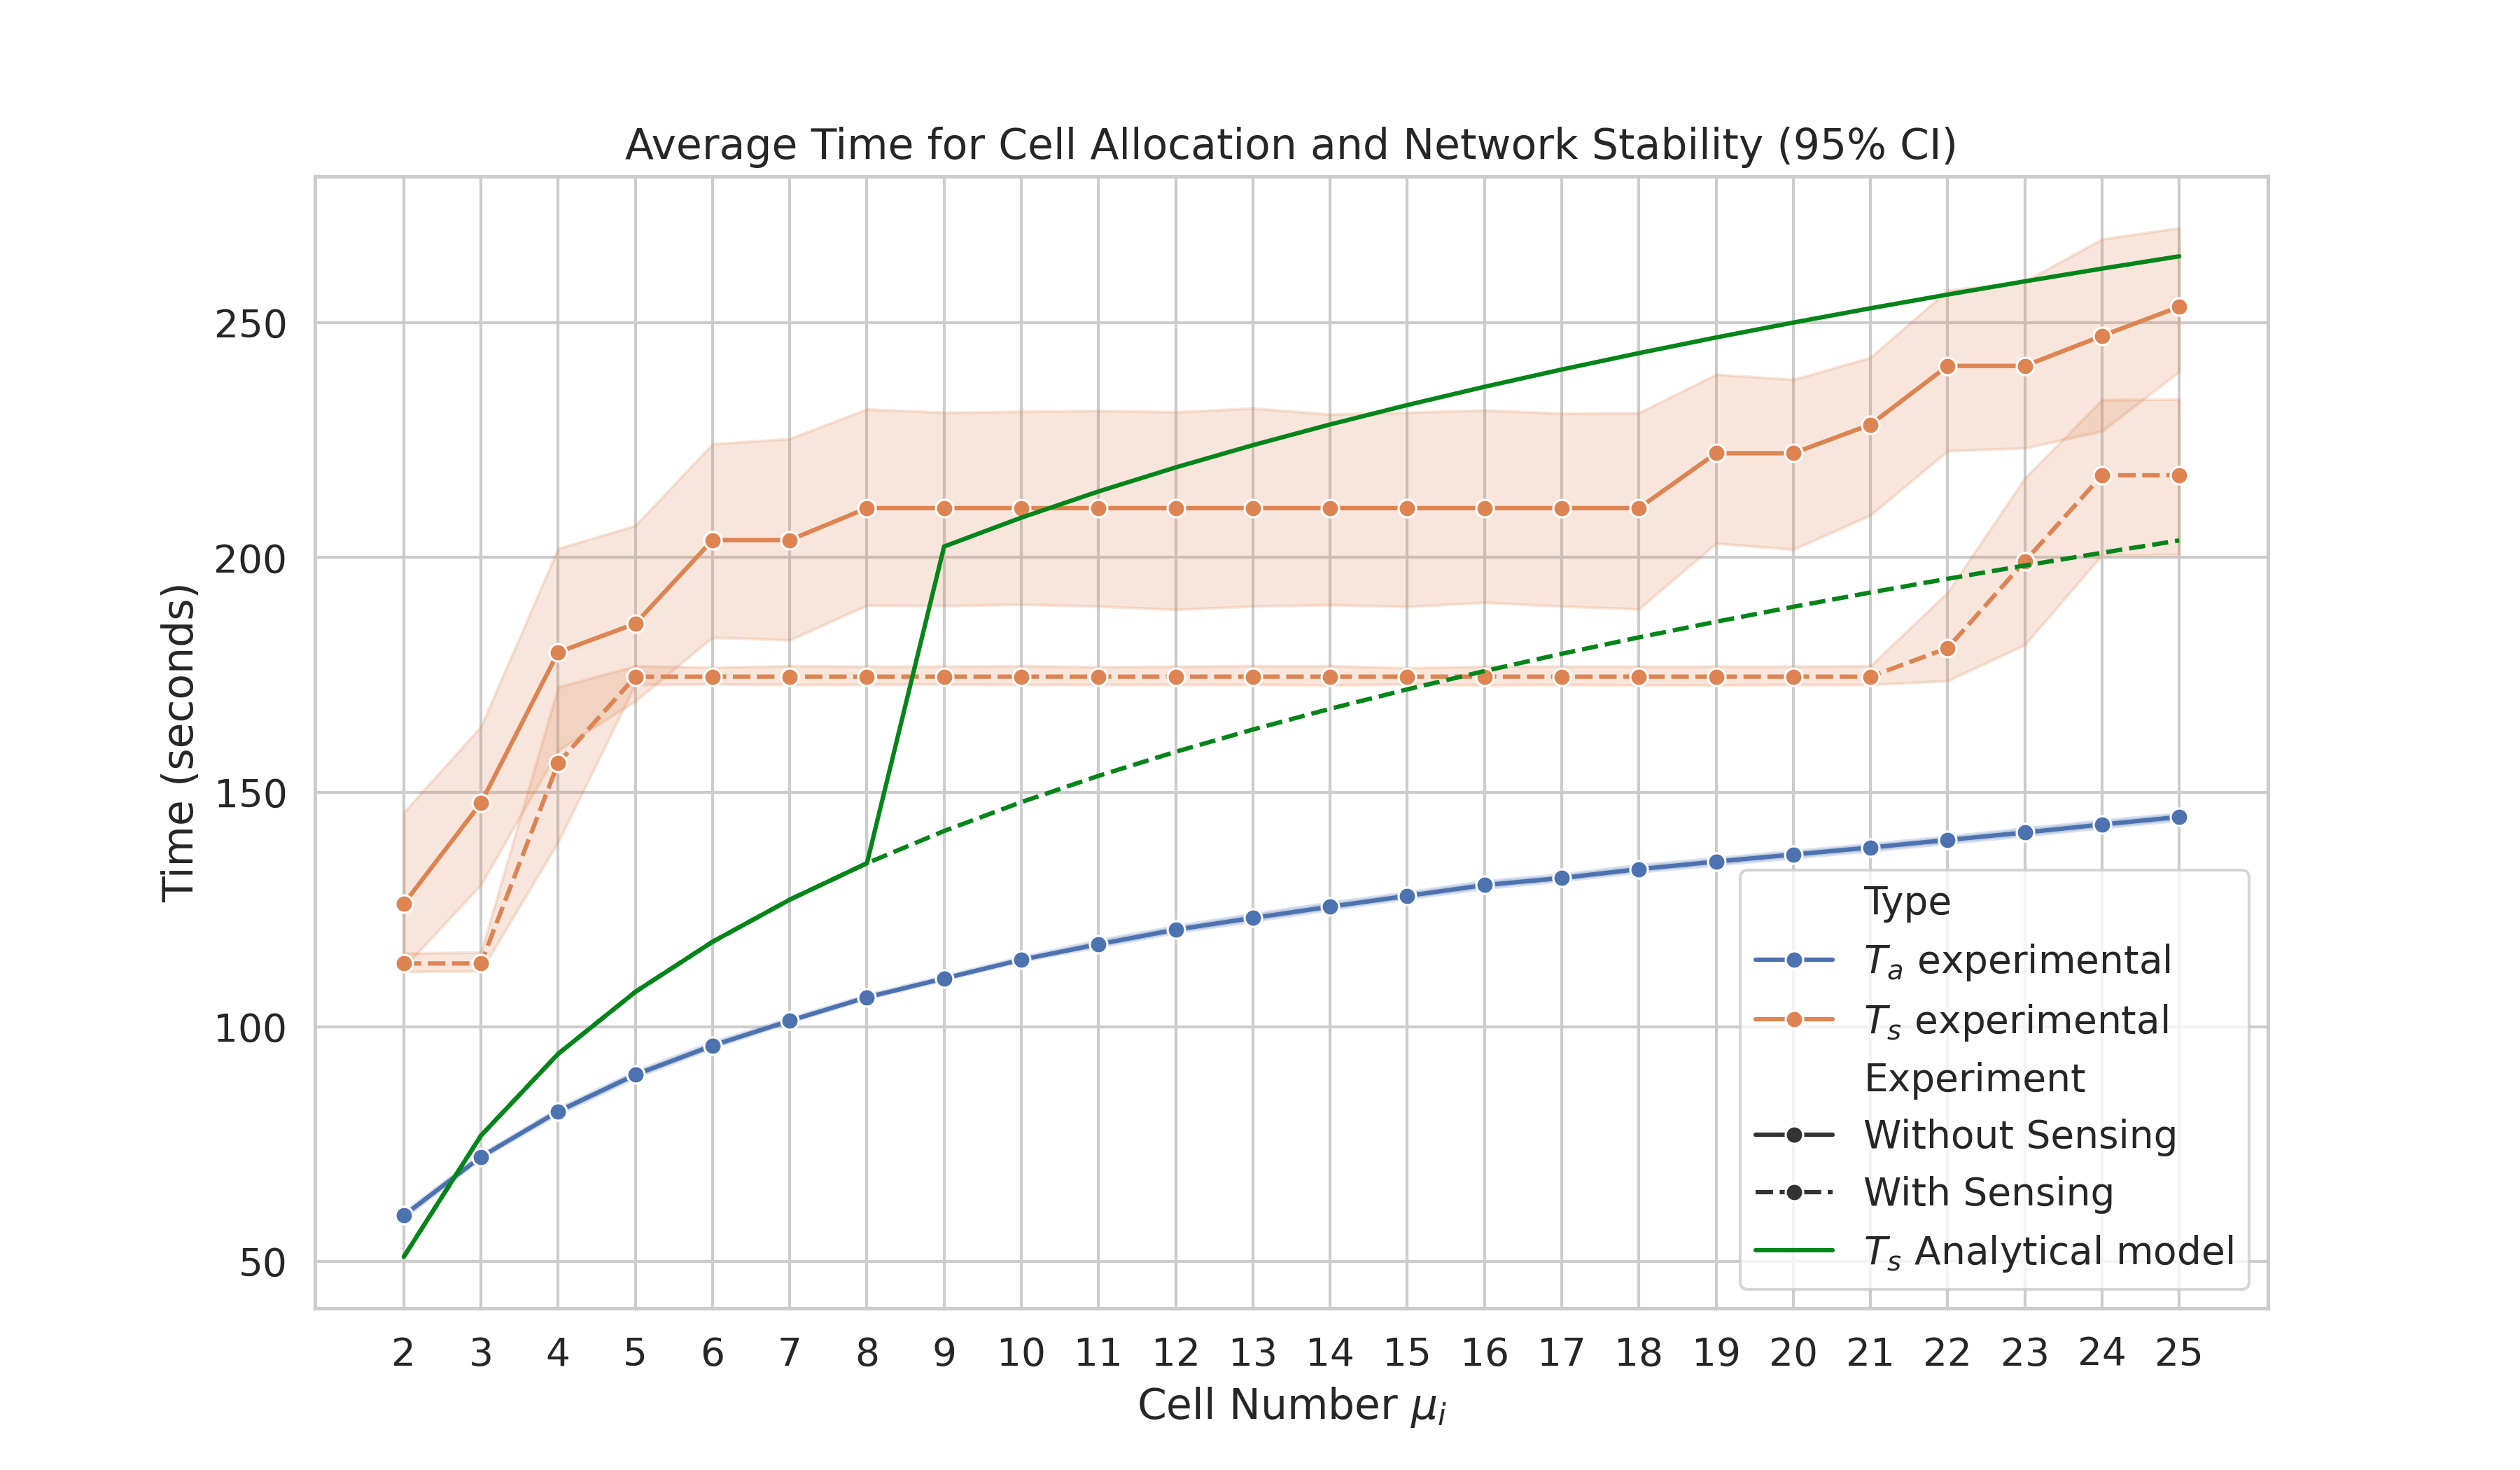
\includegraphics[width=1\textwidth]{./images/experiment4.png}
    \caption{Results of low MAX\_NUM\_CELLS with low interference.}
    \label{fig:experiment-4}
\end{figure}

Compared to Figure \ref{fig:experiment-2} with the same network interference but higher MAX\_NUM\_CELLS the values generally are lower as we expected, due to a higher frequence of cell allocations.
But the overall pattern is similar with the exception that the value plateaus at the same value from about 5 cells to 21 cells for the sensed mechanism. This is due to the mechanims of the HOUSEKEEPINGCOLLISION\_PERIOD which starts simultaneously with the cell allocation mechanism and therefore no matter how many cells are allocated if the schedule stabilizes within the same HOUSEKEEPINGCOLLISION\_PERIOD it will be measured to be stable at the same time.


\subsection*{Probability of Overlap}
To further analyse the results we look at $p_{ov}$ as \ac{KPI}. From the experiments the amount of relocations for each iteration was collected and compiled for plotting.
The following graphs compare $p_ov$ for different network interferences and under varying MAX\_NUM\_CELLS. Each value is computed from the sum of all the relocations of each cell over each iteration of an experiment and then averaged. This approach is viable since $p_ov$ only slightly varies depending on the i-th cell that is allocated.

First we consider $p_ov$ with MAX\_NUM\_CELLS being 100 comparing low and medium network interference.

\begin{figure}[H]
    \centering
    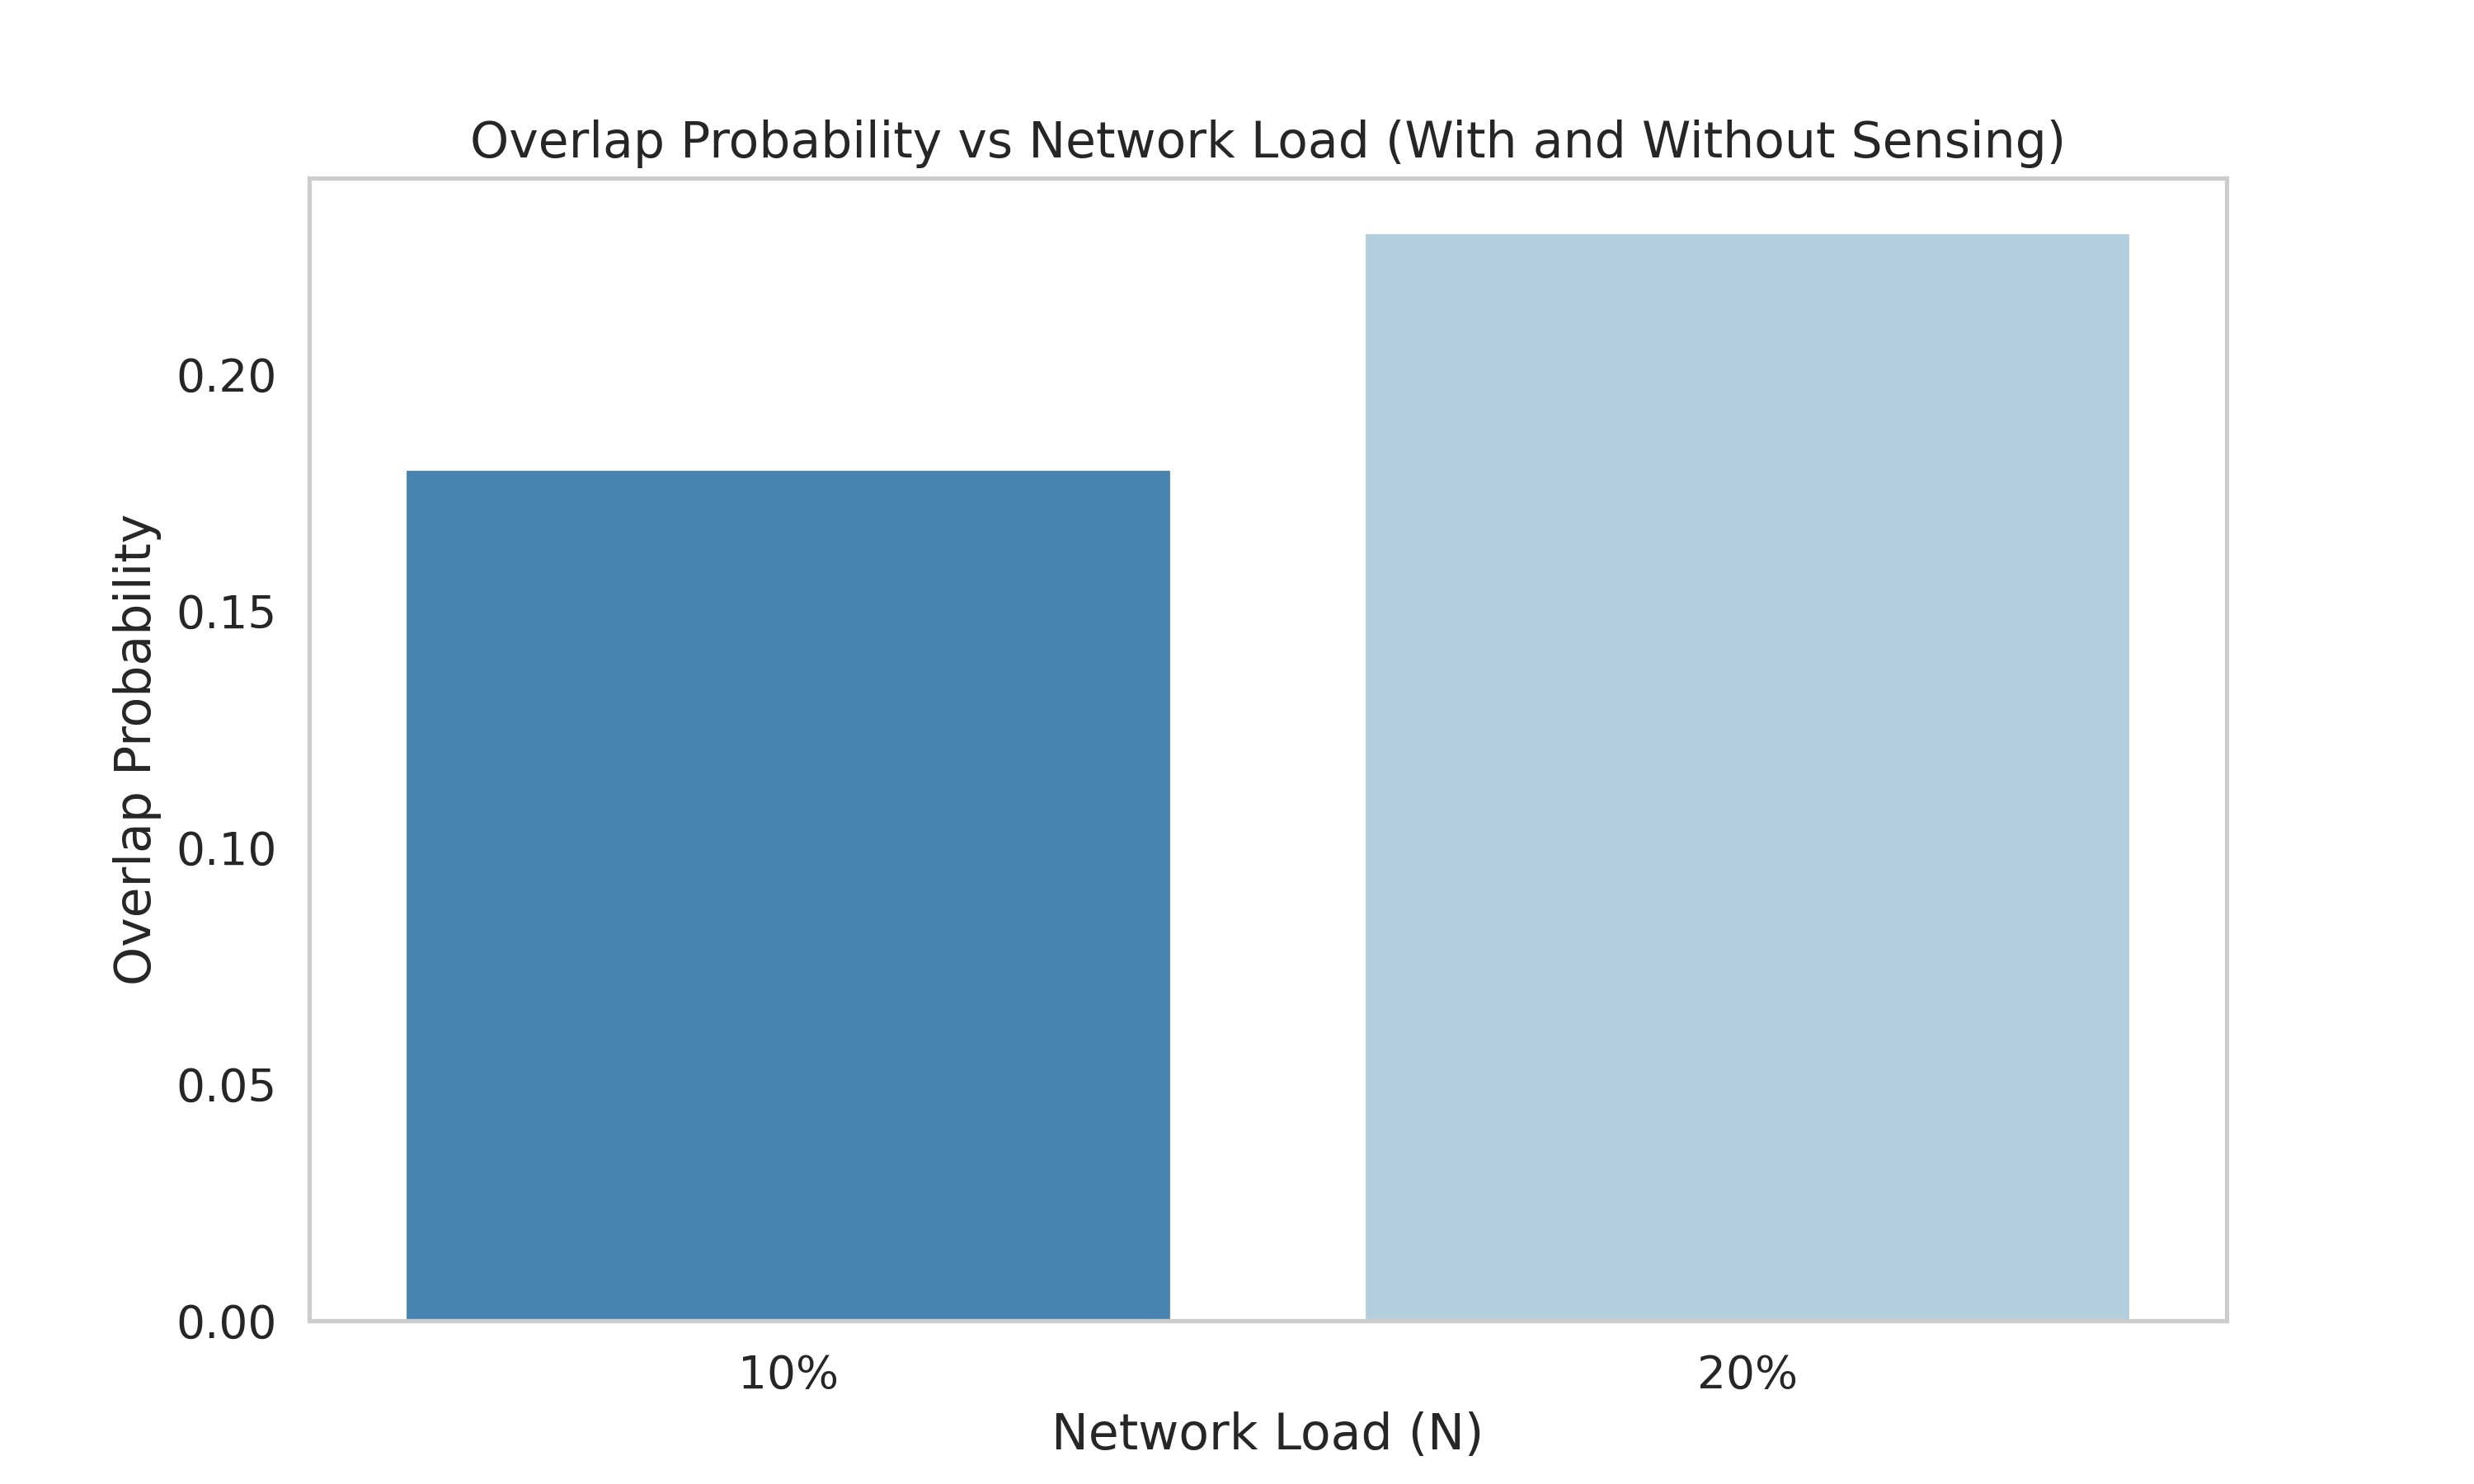
\includegraphics[width=1\textwidth]{./images/experiment_N100_pov.png}
    \caption{Experimental $p_ov$ with MAX\_NUM\_CELLS 100 comparing low and medium network interference.}
    \label{fig:pov-graph-n-100}
\end{figure}

As expected with lower network interference the probability of overlap sinks, since accoring to Equation \ref{eq:analytical-p_ov} the amount of cells occupied N goes down. For the sensing mechanism as explained in Section \ref{sec:cell-alloc-mech-sens} the expected $p_ov$ is zero which was also the result of the experiments. It is to be noted that this result is probably due to the approximative nature of the implementation described in Section \ref{sec:add-implementations} where the interfered cells were already known and the sensing operation was conducted with a success rate of 100\%.


\begin{figure}[H]
    \centering
    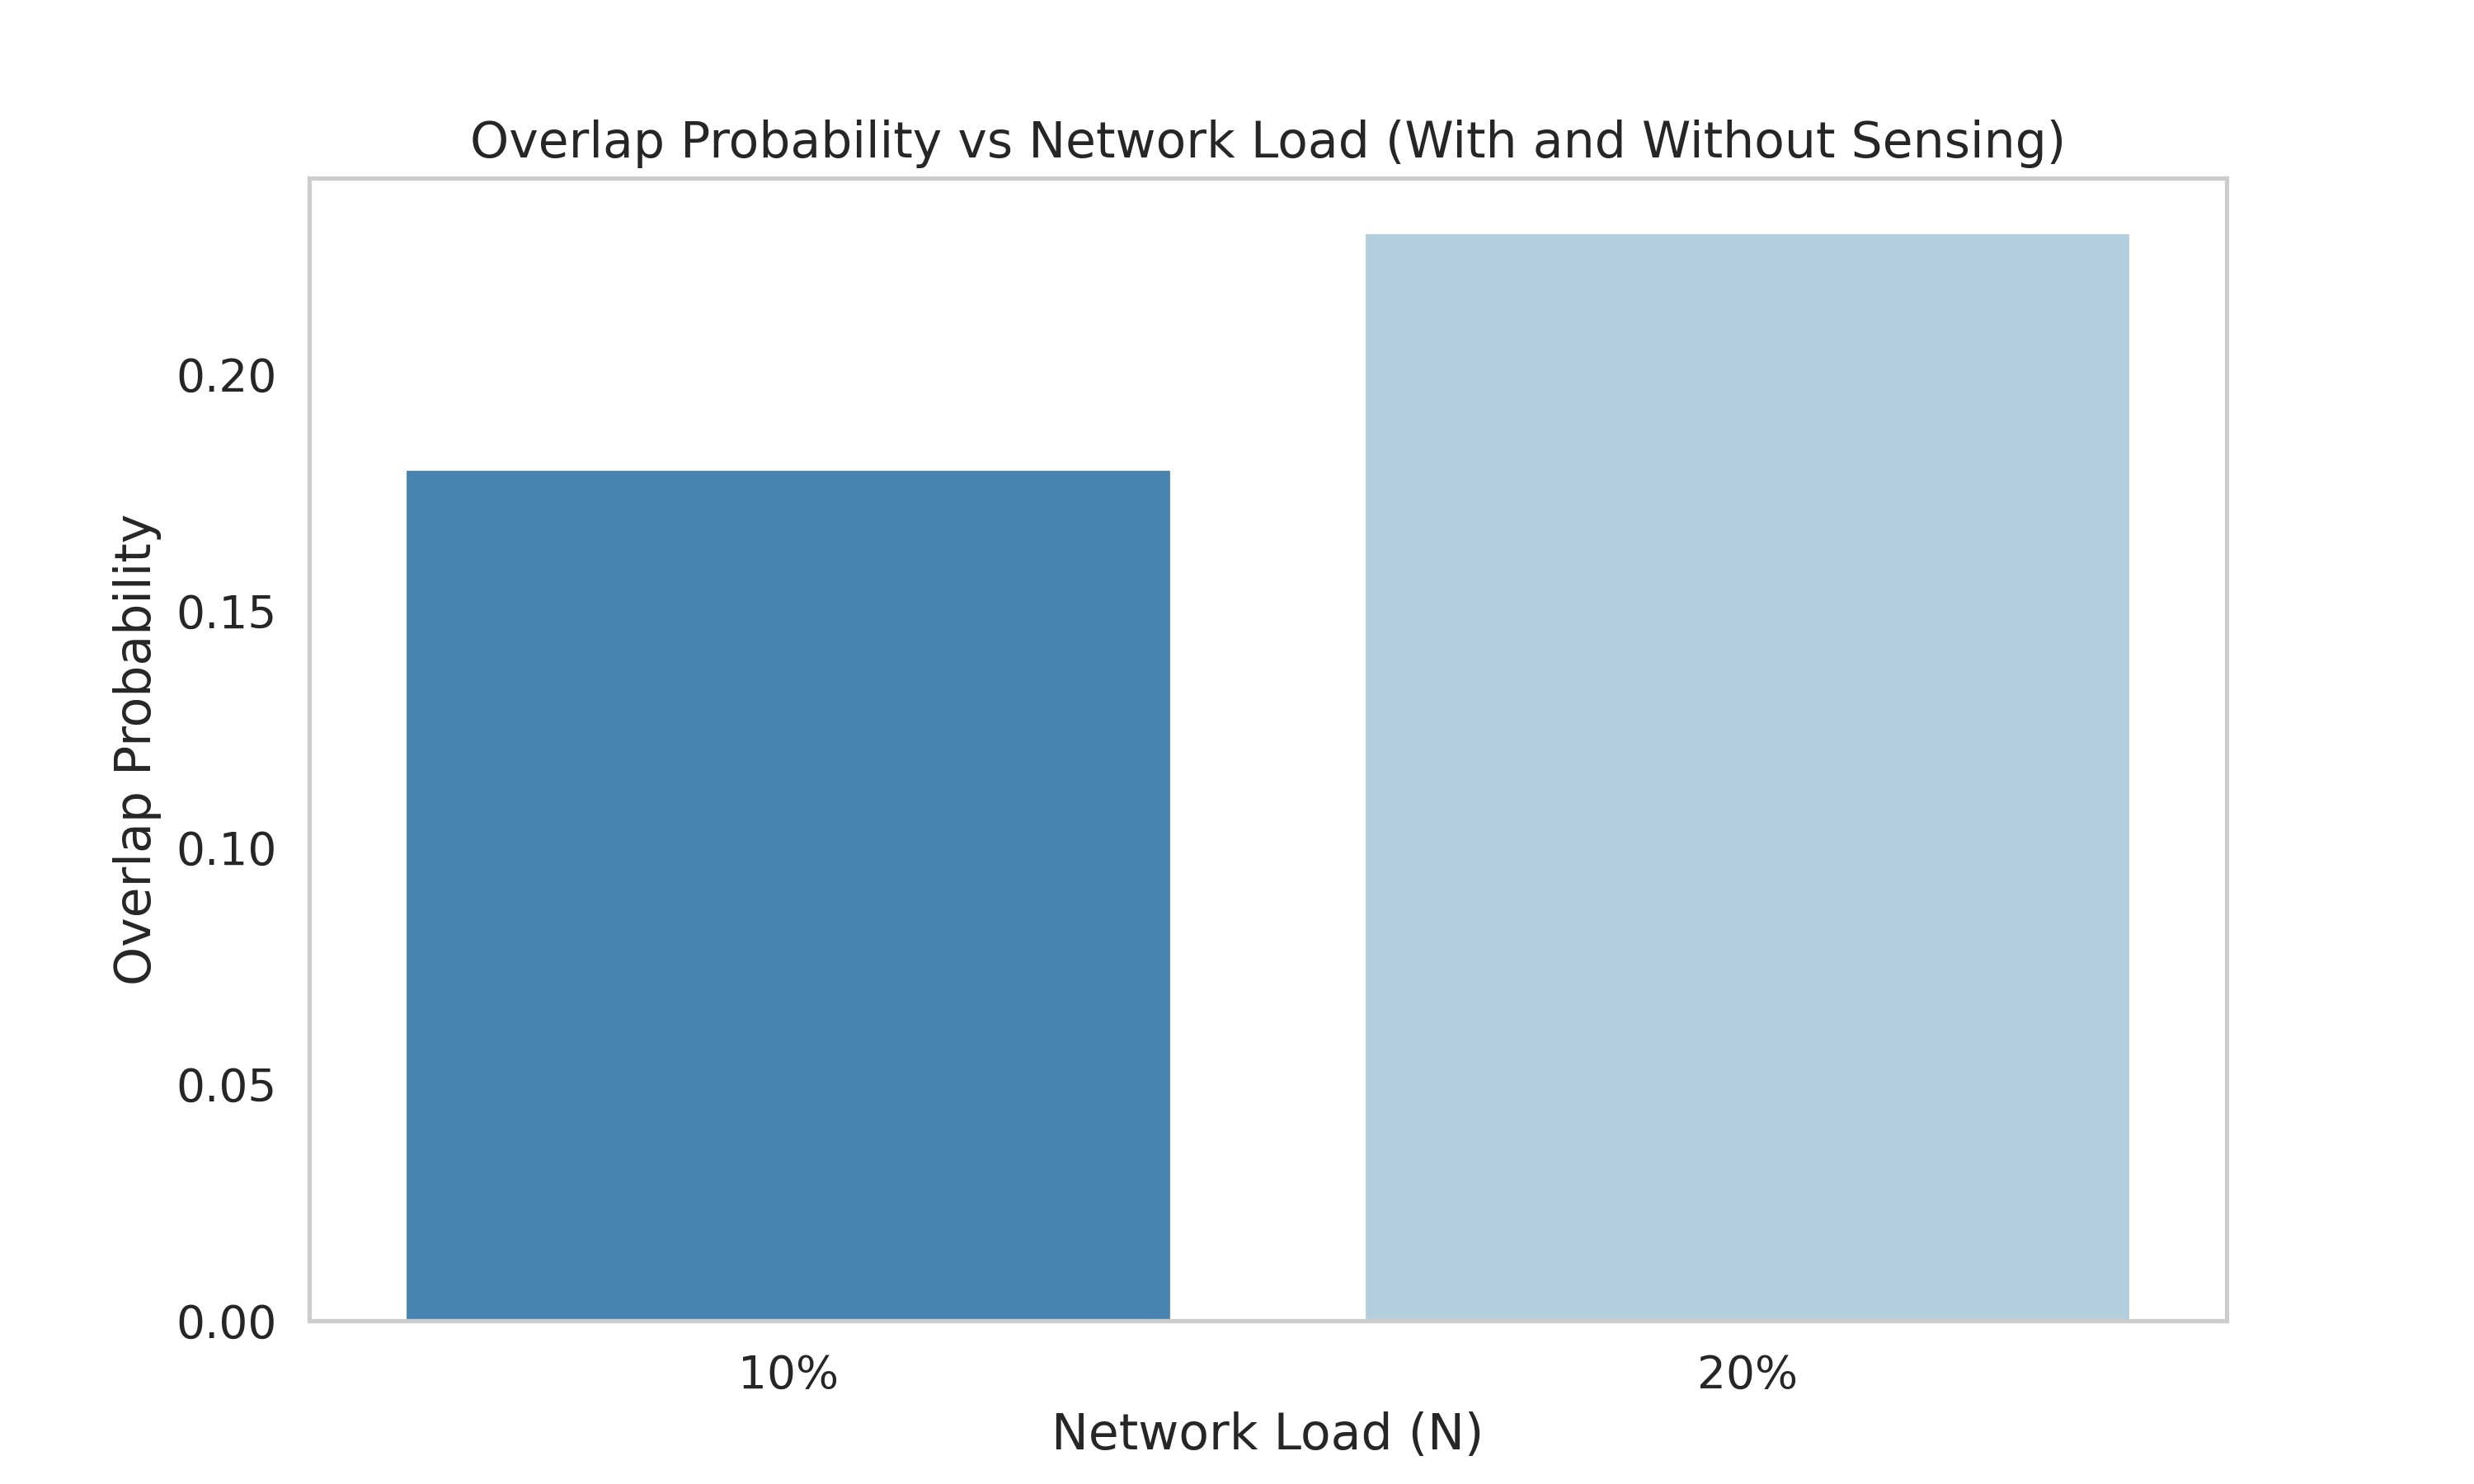
\includegraphics[width=1\textwidth]{./images/experiment_N50_pov.png}
    \caption{Experimental $p_ov$ with MAX\_NUM\_CELLS 50 comparing low and medium network interference.}
    \label{fig:pov-graph-n-50}
\end{figure}

For a MAX\_NUM\_CELLS of 50 Figure \ref{fig:pov-graph-n-50} plots the $p_ov$ for the sensing and non sensing mechanism. The probability of overlap is almost the same with the only difference being that for the sensing mechanism for a network interference of 20\% we have a slight probability of overlap. This could be just as in Figure \ref{fig:experiment-3} due to external interferences causing relocations to occour.


\chapter{Conclusion}\label{chp:conclusion}
In this work the two cell allocation mechanism were studied with varying network interference and \ac{MSF} parameters. Using an analytical model and experimental validation results show that the sensing mechanism leads to less cell overlaps resulting in less time needed to allocate a certain amount of cells and for no relocations to be necessary. It was also observed that the network interference also plays a role in cell allocation time no matter the allocation mechnism.
This work provides an analytical model to predict the time for a cell allocation and experimentally validates it showing the integrity of the model and also proving the effectiveness of experimental validation.
Although the emulation of the sensing mechanism and network interference allowed for a meaningful analysis of the cell allocation mechanisms due to simplifications some effects were not taken into account. As further work it is suggested to fully implement the sensing with cells that sense the medium for traffic, in order to find out how effective the sensing is in detecting cells that are occupied and how fast it can compile a candidate cell list without overlap. In a addition further work can focus on refining the analytical model by considering relocations of relocated cells and the effect the sensing mechanims has on \ac{6P} timout frequencies.
This work has demonstrated that the sensing cell allocation mechanism serves as a straightforward and simple enhancement to \ac{MSF}, bringing improvements in various aspects.


\listoffigures
\listoftables
\printbibliography[heading=bibintoc]

\section*{List of Acronyms}
\begin{acronym}
        % General IoT & Wireless Networking
        \acro{IoT}[IoT]{Internet of Things}
        \acro{IIoT}[IIoT]{Industrial Internet of Things}
        \acro{WSN}[WSN]{Wireless Sensor Network}
        \acro{LPWAN}[LPWAN]{Low-Power Wide-Area Network}
        \acro{MAC}[MAC]{Medium Access Control}
        \acro{PHY}[PHY]{Physical Layer}
        \acro{RF}[RF]{Radio Frequency}
        \acro{TDM}[TDM]{Time Division Multiplexing}
        \acro{FDM}[FDM]{Frequency Division Multiplexing}
        \acro{MTU}[MTU]{Maximum Transmission Unit}
        \acro{HC}[HC]{Header Compression}


    
        % 6TiSCH-Specific Acronyms
        \acro{6TiSCH}[6TiSCH]{IPv6 over the Time-Slotted Channel Hopping mode of IEEE 802.15.4e}
        \acro{6LoWPAN}[6LoWPAN]{IPv6 over Low-Power Wireless Personal Area Networks}
        \acro{6top}[6top]{6TiSCH Operation Sublayer}
        \acro{6P}[6P]{6top Protocol}
        \acro{MSF}[MSF]{Minimal Scheduling Function}
        \acro{SF}[SF]{Scheduling Function}
        \acro{OTF}[OTF]{On-The-Fly Bandwidth Reservation}
        \acro{Orchestra}[Orchestra]{An Autonomous Scheduling Function for TSCH}
        \acro{KPI}[KPI]{Key Performance Indicator}
        \acro{SAX}[SAX]{Symbolic Aggregate approXimation}
        \acro{SoC}[SoC]{System on Chip}
    
        % Routing and Network Management
        \acro{RPL}[RPL]{Routing Protocol for Low-Power and Lossy Networks}
        \acro{DAO}[DAO]{Destination Advertisement Object}
        \acro{DIO}[DIO]{DODAG Information Object}
        \acro{DODAG}[DODAG]{Destination-Oriented Directed Acyclic Graph}
        \acro{PDR}[PDR]{Packet Delivery Ratio}
        \acro{ETX}[ETX]{Expected Transmission Count}
    
        % Communication Protocols and Standards
        \acro{CoAP}[CoAP]{Constrained Application Protocol}
        \acro{OSCORE}[OSCORE]{Object Security for Constrained RESTful Environments}
        \acro{MQTT}[MQTT]{Message Queuing Telemetry Transport}
        \acro{UDP}[UDP]{User Datagram Protocol}
        \acro{ICMPv6}[ICMPv6]{Internet Control Message Protocol version 6}
        \acro{ND}[ND]{Neighbor Discovery}
        \acro{EUI64}[EUI-64]{Extended Unique Identifier 64-bit}
    
        % IEEE 802.15.4e / TSCH-Related Acronyms
        \acro{TSCH}[TSCH]{Time-Slotted Channel Hopping}
        \acro{ASN}[ASN]{Absolute Slot Number}
        \acro{CH}[CH]{Channel Hopping}
        \acro{Slotframe}[Slotframe]{A repeating structure of timeslots in TSCH}
        \acro{Cell}[Cell]{A timeslot and channel offset tuple in TSCH}
        \acro{LLN}[LLN]{Low Power and Lossy Network}
        \acro{CSMA/CA}[CSMA/CA]{Carrier-sense Multiple Access with Collision Avoidance}
        \acro{EB}[EB]{Enhanced Beacon}


    
        % Network Security and Authentication
        \acro{ACL}[ACL]{Access Control List}
        \acro{AES}[AES]{Advanced Encryption Standard}
        \acro{EAP}[EAP]{Extensible Authentication Protocol}
        \acro{PKI}[PKI]{Public Key Infrastructure}
    
        % Performance Metrics and QoS
        \acro{QoS}[QoS]{Quality of Service}
        \acro{RTT}[RTT]{Round Trip Time}
        \acro{Jitter}[Jitter]{Variation in packet delay}
        \acro{BER}[BER]{Bit Error Rate}
        \acro{PER}[PER]{Packet Error Rate}
    
        % Hardware and Energy Efficiency
        \acro{DC}[DC]{Duty Cycle}
        \acro{LQI}[LQI]{Link Quality Indicator}
        \acro{RSSI}[RSSI]{Received Signal Strength Indicator}
        \acro{EEPROM}[EEPROM]{Electrically Erasable Programmable Read-Only Memory}
        \acro{SoC}[SoC]{System on Chip}
\end{acronym}

\end{document}
